%%%%%%%%%%%%%%%%%%%%%%%%%%%%%%%%%%%%%%%%%%%%%%%%%%%%%%%%%%%%%%%%%
% Project     : AppStat Zusammenfassung FS 2018
% File        : Header.tex
% Date        : 17. Juni 2018
% Author      : Jérôme Perdrizat
% Copyright (C) 2018  J. Perdrizat
%
%    This file is free: you can redistribute it and/or modify
%    it under the terms of the GNU General Public License as published by
%    the Free Software Foundation, either version 3 of the License, or
%    (at your option) any later version, but you have to reference to the original owner.
%
%	 Additionaly the authors have to be readable in the final document.
%
%    This program is distributed in the hope that it will be useful,
%    but WITHOUT ANY WARRANTY; without even the implied warranty of
%    MERCHANTABILITY or FITNESS FOR A PARTICULAR PURPOSE.  See the
%    GNU General Public License for more details.
%
%    You should have received a copy of the GNU General Public License
%    along with this program.  If not, see <http://www.gnu.org/licenses/>.
%%%%%%%%%%%%%%%%%%%%%%%%%%%%%%%%%%%%%%%%%%%%%%%%%%%%%%%%%%%%%%%%%


\newcommand{\titleinfo}{Applied Statistics - Zusammenfassung}
\newcommand{\authorinfo}{J. Perdrizat}  % Do not remove any names! Initial authors stay first.
\newcommand{\versioninfo}{$Revision: 1 $ - powered by \LaTeX}

%%%%%%%%%%%%%%%%%%%%%%%%%%%%%%%%%%%%%%%%%%%%%
% Standard projektübergreifender Header für
% - Makros 
% - Farben
% - Mathematische Operatoren
%
% DORT NUR ERGÄNZEN, NICHTS LÖSCHEN
%%%%%%%%%%%%%%%%%%%%%%%%%%%%%%%%%%%%%%%%%%%%%

%%%%%%%%%%%%%%%%%%%%%%%%%%%%%%%%%%%%%%%%%%%%%%%%%%%%%%%%%%%%%%%%%
%
% Project     : AppStat Zusammenfassung FS 2018
% File        : Header.tex
% Date        : 17. Juni 2018
% Author      : Jérôme Perdrizat
%
%
%%%%%%%%%%%%%%%%%%%%%%%%%%%%%%%%%%%%%%%%%%%%%%%%%%%%%%%%%%%%%%%%%

\documentclass[10pt,twoside,a4paper,fleqn]{article}


%|==========================================================|
%|															|
%|  	Fonts, Grössen, weitere Zeichen				      	|
%|															|
%|==========================================================|
\usepackage[utf8]{inputenc}       %für Umlaute
\usepackage[ngerman]{babel}
\usepackage{amsmath,amssymb}



%|==========================================================|
%|															|
%|  				verwendete Pakete				      	|
%|				(alphabetisch absteigend)					|
%|==========================================================|
\usepackage{array}
\usepackage{array}
\usepackage{circuitikz}
\usepackage{enumitem}
\usepackage{graphics}
\usepackage{hyperref}
\usepackage{lastpage}
\usepackage{longtable}
\usepackage{mathtools}
\usepackage{multicol} %Intermix single and mulltiple collums­
\usepackage{multirow}
\usepackage{pdfpages}
\usepackage{rotating} % Rotation tools, including rotated fullpage floats
\usepackage{siunitx}
\usepackage{subfig}
\usepackage{tabularx}
\usepackage{todonotes}


%|==========================================================|
%|															|
%|  	Seiten Formatierungsinformationen					|
%|			inkl. Kopf- und Fusszeile				      	|
%|															|
%|==========================================================|

\usepackage{geometry}
\usepackage{fancyhdr}
\usepackage{fancybox}

%Seitenränder
\geometry{
	left 	= 1cm
	,right 	= 1 cm
	,top	= 1 cm
	,bottom = 1 cm
	,includeheadfoot}

%pdf info
\hypersetup{pdfauthor={\authorinfo},pdftitle={\titleinfo},colorlinks=false}
\author{\authorinfo}
\title{\titleinfo}

%Kopf- und Fusszeile
\pagestyle{fancy}
\fancyhf{}

%Linien oben und unten
\renewcommand{\headrulewidth}{0.5pt} 
\renewcommand{\footrulewidth}{0.5pt}
\fancyhead[L]{\titleinfo{ }\tiny{(\versioninfo)}}

%Kopfzeile rechts bzw. aussen
\fancyhead[R]{Seite \thepage { }von \pageref{LastPage}}

%Fusszeile links bzw. innen
\fancyfoot[L]{\footnotesize{\authorinfo}}

%Fusszeile rechts bzw. ausen
\fancyfoot[R]{\footnotesize{\today}}



%|==========================================================|
%|															|
%|  	Weitere Formatierungsinformationen 					|
%|					(Paketbezogen)							|
%|==========================================================|



%|==========================================================|
%|															|
%|  		Makros & anderer Low-Level bastel				|
%|					(Paketbezogen)							|
%|==========================================================|
\makeatletter
%% Makros für Titel, Autor und Datum 
%% Dank diesem Makro stehen Titel, Autor und Datum überall im Dokument zur verfügung
%% Date hat zudem den Default-Wert \today
\def\@Title{}
\def\@Author{}
\def\@Date{\today}
\newcommand{\Title}{\@Title}
\newcommand{\Author}{\@Author}
\newcommand{\Date}{\@Date}
\AtBeginDocument{%
	\let\@Title\@title
	\let\@Author\@author
	\let\@Date\@date
}






\ifx\GUARDenumitem\undefined
\def\GUARDenumitem{}

\usepackage{enumitem}


\setlist{itemsep=-2pt}
\setlist{parsep=-2pt}

\fi
\ifx \GUARDhsrColors \undefined
\def\GUARDhsrColors{}

\usepackage{xcolor}

\definecolor{HSRWhite}{cmyk}{0,0,0,0}

\definecolor{HSRBlue}{cmyk}{1,0.4,0,0.2}
\definecolor{HSRBlue80}{cmyk}{0.8,0.32,0,0.16}
\definecolor{HSRBlue60}{cmyk}{0.6,0.24,0,0.12}
\definecolor{HSRBlue40}{cmyk}{0.4,0.16,0,0.08}
\definecolor{HSRBlue20}{cmyk}{0.2,0.08,0,0.04}

\definecolor{HSRLightGray}{cmyk}{0,0,0,0.30}
\definecolor{HSRLightGray80}{cmyk}{0,0,0,0.24}
\definecolor{HSRLightGray60}{cmyk}{0,0,0,0.18}
\definecolor{HSRLightGray40}{cmyk}{0,0,0,0.12}
\definecolor{HSRLightGray20}{cmyk}{0,0,0,0.06}

\definecolor{HSRSchwarz}{cmyk}{0,0,0,1}
\definecolor{HSRSchwarz80}{cmyk}{0,0,0,0.8}
\definecolor{HSRSchwarz60}{cmyk}{0,0,0,0.6}
\definecolor{HSRSchwarz40}{cmyk}{0,0,0,0.4}
\definecolor{HSRSchwarz20}{cmyk}{0,0,0,0.2}

\definecolor{HSRHematite}{cmyk}{0.6,1,0.4,0.2}
\definecolor{HSRHematite80}{cmyk}{0.48,0.80,0.32,0.16}
\definecolor{HSRHematite60}{cmyk}{0.36,0.60,0.24,0.12}
\definecolor{HSRHematite40}{cmyk}{0.24,0.40,0.16,0.08}
\definecolor{HSRHematite20}{cmyk}{0.12,0.20,0.08,0.04}

\definecolor{HSRLakeGreen}{cmyk}{0.70,0.30,0.45,0.05}
\definecolor{HSRLakeGreen80}{cmyk}{0.56,0.24,0.36,0.03}
\definecolor{HSRLakeGreen60}{cmyk}{0.42,0.18,0.27,0.02}
\definecolor{HSRLakeGreen40}{cmyk}{0.28,0.06,0.13,0.06}
\definecolor{HSRLakeGreen20}{cmyk}{0.14,0.06,0.09,0.01}

\definecolor{HSRReed}{cmyk}{0.10,0.25,0.45,0.60}
\definecolor{HSRReed80}{cmyk}{0.08,0.20,0.36,0.48}
\definecolor{HSRReed60}{cmyk}{0.06,0.15,0.27,0.36}
\definecolor{HSRReed40}{cmyk}{0.04,0.10,0.18,0.24}
\definecolor{HSRReed20}{cmyk}{0.02,0.05,0.09,0.12}

\definecolor{HSRPetrol}{cmyk}{1,0.18,0,0.45}
\definecolor{HSRPetrol80}{cmyk}{0.64,0.08,0.12,0.32}
\definecolor{HSRPetrol60}{cmyk}{0.48,0.06,0.09,0.24}
\definecolor{HSRPetrol40}{cmyk}{0.32,0.04,0.06,0.16}
\definecolor{HSRPetrol20}{cmyk}{0.16,0.02,0.03,0.08}

\definecolor{HSRBasswood}{cmyk}{0.25,0.05,0.70,0.15}
\definecolor{HSRBasswood80}{cmyk}{0.20,0.04,0.56,0.12}
\definecolor{HSRBasswood60}{cmyk}{0.15,0.03,0.42,0.09}
\definecolor{HSRBasswood40}{cmyk}{0.10,0.02,0.28,0.06}
\definecolor{HSRBasswood20}{cmyk}{0.05,0.01,0.14,0.03}


\fi
\ifx\GUARDhyperref\undefined
\def\GUARDhyperref{}

\ifx \GUARDhsrColors \undefined
\def\GUARDhsrColors{}

\usepackage{xcolor}

\definecolor{HSRWhite}{cmyk}{0,0,0,0}

\definecolor{HSRBlue}{cmyk}{1,0.4,0,0.2}
\definecolor{HSRBlue80}{cmyk}{0.8,0.32,0,0.16}
\definecolor{HSRBlue60}{cmyk}{0.6,0.24,0,0.12}
\definecolor{HSRBlue40}{cmyk}{0.4,0.16,0,0.08}
\definecolor{HSRBlue20}{cmyk}{0.2,0.08,0,0.04}

\definecolor{HSRLightGray}{cmyk}{0,0,0,0.30}
\definecolor{HSRLightGray80}{cmyk}{0,0,0,0.24}
\definecolor{HSRLightGray60}{cmyk}{0,0,0,0.18}
\definecolor{HSRLightGray40}{cmyk}{0,0,0,0.12}
\definecolor{HSRLightGray20}{cmyk}{0,0,0,0.06}

\definecolor{HSRSchwarz}{cmyk}{0,0,0,1}
\definecolor{HSRSchwarz80}{cmyk}{0,0,0,0.8}
\definecolor{HSRSchwarz60}{cmyk}{0,0,0,0.6}
\definecolor{HSRSchwarz40}{cmyk}{0,0,0,0.4}
\definecolor{HSRSchwarz20}{cmyk}{0,0,0,0.2}

\definecolor{HSRHematite}{cmyk}{0.6,1,0.4,0.2}
\definecolor{HSRHematite80}{cmyk}{0.48,0.80,0.32,0.16}
\definecolor{HSRHematite60}{cmyk}{0.36,0.60,0.24,0.12}
\definecolor{HSRHematite40}{cmyk}{0.24,0.40,0.16,0.08}
\definecolor{HSRHematite20}{cmyk}{0.12,0.20,0.08,0.04}

\definecolor{HSRLakeGreen}{cmyk}{0.70,0.30,0.45,0.05}
\definecolor{HSRLakeGreen80}{cmyk}{0.56,0.24,0.36,0.03}
\definecolor{HSRLakeGreen60}{cmyk}{0.42,0.18,0.27,0.02}
\definecolor{HSRLakeGreen40}{cmyk}{0.28,0.06,0.13,0.06}
\definecolor{HSRLakeGreen20}{cmyk}{0.14,0.06,0.09,0.01}

\definecolor{HSRReed}{cmyk}{0.10,0.25,0.45,0.60}
\definecolor{HSRReed80}{cmyk}{0.08,0.20,0.36,0.48}
\definecolor{HSRReed60}{cmyk}{0.06,0.15,0.27,0.36}
\definecolor{HSRReed40}{cmyk}{0.04,0.10,0.18,0.24}
\definecolor{HSRReed20}{cmyk}{0.02,0.05,0.09,0.12}

\definecolor{HSRPetrol}{cmyk}{1,0.18,0,0.45}
\definecolor{HSRPetrol80}{cmyk}{0.64,0.08,0.12,0.32}
\definecolor{HSRPetrol60}{cmyk}{0.48,0.06,0.09,0.24}
\definecolor{HSRPetrol40}{cmyk}{0.32,0.04,0.06,0.16}
\definecolor{HSRPetrol20}{cmyk}{0.16,0.02,0.03,0.08}

\definecolor{HSRBasswood}{cmyk}{0.25,0.05,0.70,0.15}
\definecolor{HSRBasswood80}{cmyk}{0.20,0.04,0.56,0.12}
\definecolor{HSRBasswood60}{cmyk}{0.15,0.03,0.42,0.09}
\definecolor{HSRBasswood40}{cmyk}{0.10,0.02,0.28,0.06}
\definecolor{HSRBasswood20}{cmyk}{0.05,0.01,0.14,0.03}


\fi

\usepackage{hyperref}
\hypersetup{
  pdfstartview={FitH}, % fits the width of the page to the window
  pdfauthor={\Author},
  pdfcreator={\Author},
  pdfproducer={\Author},
  pdftitle={\Title},
  colorlinks=false,
  linkcolor=HSRBlue,
  citecolor=HSRReed,
  filecolor=HSRLake,
  urlcolor=HSRHematite
}

\fi
\ifx\GUARDlistings\undefined
\def\GUARDlistings{}

\usepackage{listings}
\lstdefinestyle{Java}{ numbers=left,
  belowcaptionskip=1\baselineskip,
  breaklines=true,
  frame=L,
  xleftmargin=10pt,
  language=Java,
  showstringspaces=false,
  basicstyle=\footnotesize\ttfamily,
  keywordstyle=\bfseries\color{green!40!black},
  commentstyle=\itshape\color{purple!40!black},
  identifierstyle=\color{blue},
  stringstyle=\color{orange},
  numberstyle=\ttfamily\tiny,
  tabsize=2
}

\lstdefinestyle{SQL}{
  numbers=none,
  belowcaptionskip=1\baselineskip,
  breaklines=true,
  xleftmargin=10pt,
  language=SQL,
  showstringspaces=false,
  basicstyle=\footnotesize\ttfamily,
  keywordstyle=\bfseries\color{green!40!black},
  commentstyle=\itshape\color{purple!40!black},
  identifierstyle=\color{blue},
  stringstyle=\color{orange},,
  tabsize=2
}

\lstdefinestyle{C}{
  numbers=left,
  belowcaptionskip=1\baselineskip,
  breaklines=true,
  frame=L,
  xleftmargin=10pt,
  language=C,
  showstringspaces=false,
  basicstyle=\footnotesize\ttfamily,
  keywordstyle=\bfseries\color{green!40!black},
  commentstyle=\itshape\color{purple!40!black},
  identifierstyle=\color{blue},
  stringstyle=\color{orange},
  numberstyle=\ttfamily\tiny,
  tabsize=2
}

\lstdefinestyle{Cpp}{
  numbers=left,
  belowcaptionskip=1\baselineskip,
  breaklines=true,
  frame=L,
  xleftmargin=10pt,
  language=C++,
  showstringspaces=false,
  basicstyle=\footnotesize\ttfamily,
  keywordstyle=\bfseries\color{green!40!black},
  commentstyle=\itshape\color{purple!40!black},
  identifierstyle=\color{blue},
  stringstyle=\color{orange},
  numberstyle=\ttfamily\tiny,
  tabsize=2
}

\lstdefinestyle{Csharp}{
  numbers=left,
  belowcaptionskip=1\baselineskip,
  breaklines=true,
  frame=L,
  xleftmargin=10pt,
  language=[Sharp]C,
  showstringspaces=false,
  basicstyle=\footnotesize\ttfamily,
  keywordstyle=\bfseries\color{green!40!black},
  commentstyle=\itshape\color{purple!40!black},
  identifierstyle=\color{blue},
  stringstyle=\color{orange},
  numberstyle=\ttfamily\tiny,
  tabsize=2
}

\lstdefinestyle{Matlab}{
  numbers=left,
  belowcaptionskip=1\baselineskip,
  breaklines=true,
  frame=L,
  xleftmargin=10pt,
  language=Matlab,
  showstringspaces=false,
  basicstyle=\footnotesize\ttfamily,
  keywordstyle=\bfseries\color{green!40!black},
  commentstyle=\itshape\color{purple!40!black},
  identifierstyle=\color{blue},
  stringstyle=\color{orange},
  numberstyle=\ttfamily\tiny,
  tabsize=2
}

\lstdefinestyle{VHDL}{
  numbers=left,
  belowcaptionskip=1\baselineskip,
  breaklines=true,
  frame=L,
  xleftmargin=0pt,
  language=VHDL,
  showstringspaces=false,
  basicstyle=\footnotesize\ttfamily,
  keywordstyle=\bfseries\color{green!40!black},
  commentstyle=\itshape\color{purple!40!black},
  identifierstyle=\color{blue},
  stringstyle=\color{orange},
  numberstyle=\ttfamily\tiny,
  tabsize=2
}

\lstdefinestyle{ASM}{
  numbers=left,
  belowcaptionskip=1\baselineskip,
  breaklines=true,
  frame=L,
  xleftmargin=10pt,
  language=[x86masm]Assembler,
  showstringspaces=false,
  basicstyle=\footnotesize\ttfamily,
  keywordstyle=\bfseries\color{green!40!black},
  commentstyle=\itshape\color{purple!40!black},
  identifierstyle=\color{blue},
  stringstyle=\color{orange},
  numberstyle=\ttfamily\tiny,
  tabsize=2
}

\lstdefinestyle{R}{
  numbers=left,
  belowcaptionskip=1\baselineskip,
  breaklines=true,
  frame=L,
  xleftmargin=10pt,
  aboveskip=-5pt,
  language=R,
  showstringspaces=false,
  basicstyle=\footnotesize\ttfamily,
  keywordstyle=\bfseries\color{green!40!black},
  commentstyle=\itshape\color{purple!40!black},
  identifierstyle=\color{blue},
  stringstyle=\color{orange},
  numberstyle=\ttfamily\tiny,
  tabsize=1
}
\fi

\ifx\GUARDmathe\undefined
\def\GUARDmathe{}

\usepackage{amssymb}
% Das mathtools package ist eine Erweiterung zum amsmath package.
% Das amsmath package wird dabei automatisch geladen
\usepackage{mathtools}


% Package mit vielen weiteren Mathe Symbolen
% http://www.ctan.org/tex-archive/fonts/mathabx
\usepackage{mathabx}

% This package defines commands to access bold math symbols. The basic command
% is \bm which may be used to make the math expression in its argument be typeset
% using bold fonts.
\usepackage{bm}

% Package for differentiation operators
\usepackage{esdiff}

\fi
\usepackage{tikz}
\usetikzlibrary{trees}
\usetikzlibrary{positioning}
\ifx\BIBLATEXsetings\undefined
\def\BIBLATEXsetings{}

%|==========================================================|
%|															|
%|  	Pakete, Commands und Links für Quellenverzeichnis  	|
%|															|
%|==========================================================|
\usepackage	[backend=bibtex,			%Format der Referenz
			style=ieee]{biblatex}		%Ausführung des Verzeichnises
\addbibresource{./References.bib}
\usepackage{hyperref}
\usepackage{etoolbox}
\apptocmd{\UrlBreaks}{\do\f\do\m}{}{}
\setcounter{biburllcpenalty}{9000}% Kleinbuchstaben
\setcounter{biburlucpenalty}{9000}% Großbuchstaben

\fi 

\begin{document}
\small %Schriftgrösse auf small setzen
\tableofcontents
\section{Vorwort}
Dieses Dokument enthält sowohl aus den Unterlagen von Herr Steiner-Curtis \cite{C:SteinerCurtis} wie auch aus Herr Ruckstuhls Folien \cite{C:Ruckstuhl} teilweise übernommenen Sätze. Die von den Skripts verwendeten Grafiken sind jeweils mit dem Quellenangaben versehen. Die gesamte Zusammenfassung basiert auf diesen Dokumenten. 
\newpage
\section{SPC - Statistische Prozess- und Qualitätskontrolle}

\subsection{Einleitung}
\begin{itemize}
	\item Qualität = Gebrauchstauglichkeit
	\begin{itemize}
		\item Umgekehrt Proportional zur Variabilität
	\end{itemize}
	\item Wichtigste Tool: Die glorreichen Sieben
	\begin{itemize}
		\item[1.] Histogramm
		\item[2.] Check-Sheet (siehe Kapitel \ref{subsubsec:Kontrollblatt})
		\item[3.] Defect Concentration Diagramm (siehe Kapitel \ref{subsubsec:DefectConcentrationDiagramm})
		\item[4.] Pareto Chart (siehe Kapitel \ref{subsubsec:ParetoChart})
		\item[5.] Cause-and-Effect Diagramm (siehe Kapitel \ref{subsubsec:UrsacheWirkungsDiagramm})
		\item[6.] Kontrollkarte (siehe Kapitel \ref{subsec:Kontrollkarte})
		\item[7.] Streudiagramm
	\end{itemize}
\end{itemize}

\subsection{Basics}
\begin{itemize}
	\item Mittelwert mehrer Messwerte wird mit einem Querstrich bezeichnet, siehe z.B. Formel \ref{eq:Kontrollkarte1}.
	\item Ein geschätzer wert wird mit $\hat{ }$ bezeichnet (z.B. $\hat{\sigma}$
	\begin{itemize}
		\item Der exakte Wert ist nicht bekannt, wir schätzen mit werten aus der Vergangenheit
	\end{itemize}
	\item Nullhypothese $H_0$
	\begin{itemize}
		\item Annahme der 0-Hypothese: Prozess ist unter Kontrolle
		\item Ablehunung der 0-Hypothese: Prozess ist nicht unter Kontrolle
	\end{itemize}
\end{itemize}


\subsubsection{Kontrollblatt (Check-Sheet)}
\label{subsubsec:Kontrollblatt}
\begin{itemize}
	\item Formular zur Registrierung und Zählung möglicher Probleme
	\item Erfasst Ursachen und deren Auftreten für ein bestimmtes Ereignis (kann auch über verschiedene Zeitpunkte gemacht werden)
	\item Beispiel siehe Tabelle \ref{tab:CheckSheet}
\end{itemize}

\begin{table}[h!]
	\centering
	\begin{tabular}{l | c c c c | c}
		Ursachen					& \multicolumn{4}{c}{Unterbrechungen pro Quartal} 	&\\
									&1.		&2.		& 3.	&4.							&total\\\hline
		Telefon fallen lassen		&1		&0		&0		&2							&3\\
		Akku leer					&3		&3		&2		&4							&12\\
		Tunnelfahrt					&12		&10		&13		&9							&44\\
		Taste gedrückt				&1		&1		&0		&3							&5\\
		Unfall produziert			&1		&0		&0		&0							&1\\
		Telefon kaputt				&1		&0		&2		&1							&4\\
		kein offensichtlicher Grund	&3		&4		&3		&5							&15
	\end{tabular}
	\label{tab:CheckSheet}
	\caption{Beispiel eines Kontrollblattes \textit{Quelle:} \cite{C:CurtisSkriptCause}}
\end{table}


\subsubsection{Defect Concentration Diagramm}
\label{subsubsec:DefectConcentrationDiagramm}
\begin{itemize}
	\item Grafisches Pendant zum Kontrollblatt
	\item Auch Location Plot genannt
	\item Zeigt grafisch Orte des Auftretens verschiedener Fehler (Beispiel: Abbildung \ref{fig:DefectConcentration}
\end{itemize}
\begin{figure}[!h]
	\centering
	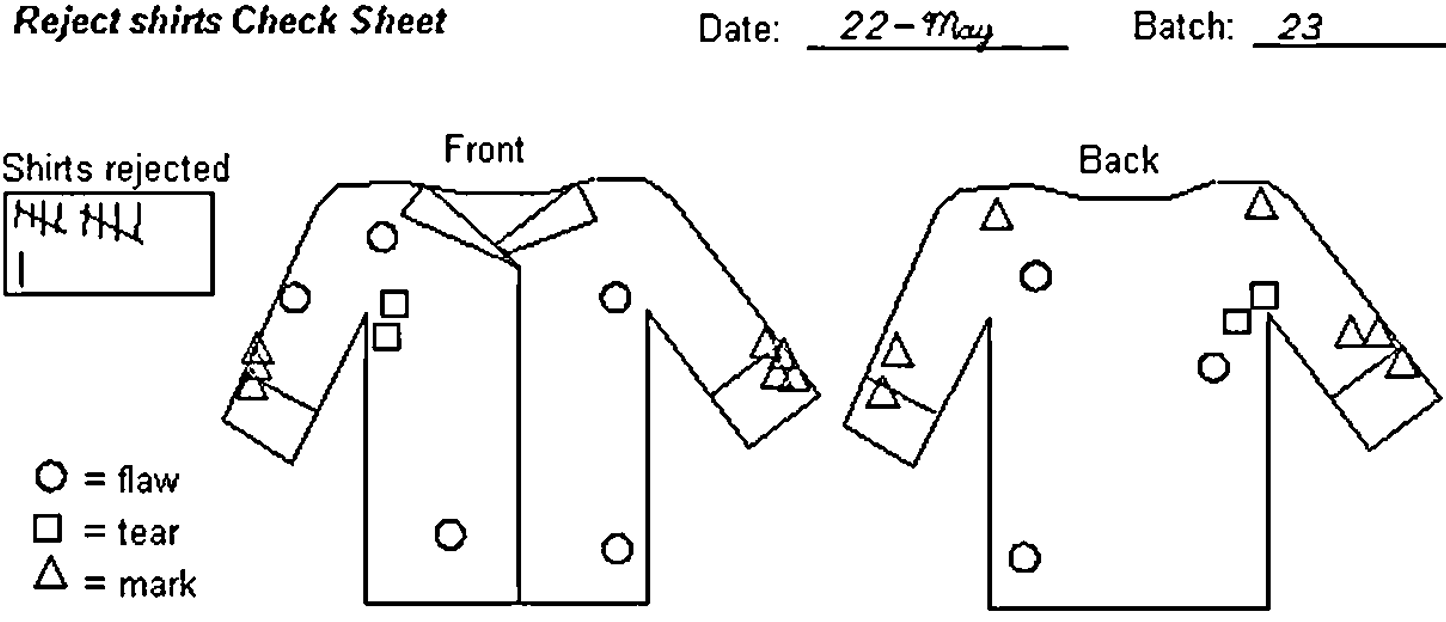
\includegraphics[width=0.5\linewidth]{figures/DefectConcentration}
	\caption{Ein Defect Concentration Diagramm \textit{Quelle:}\cite{C:DefectConcentration}}
	\label{fig:DefectConcentration}
\end{figure}

\subsubsection{Pareto-Chart}
\label{subsubsec:ParetoChart}
\begin{itemize}
	\item Bekannter unter dem Namen \glqq 80-20-Prinzip\grqq
	\begin{itemize}
		\item Wie viel Prozent des Resultats werden mit wie vielen Prozent des Einsatzes erreicht?
	\end{itemize}
	\item Mit einem kleinen Teil der eingesetzten Mittel bereits eine grosse Wirkung erzielen
	\item Pareto-Chart ist eine Spezielle Art des Histrogramms
	\begin{itemize}
		\item Histogramm und im gleichen Plott (auch auf gleicher Achsskalierung) die Summe aller bis zu diesem Punkt eingetragenen Histogramm-Werten
	\end{itemize}
\end{itemize}
\begin{figure}[!h]
	\centering
	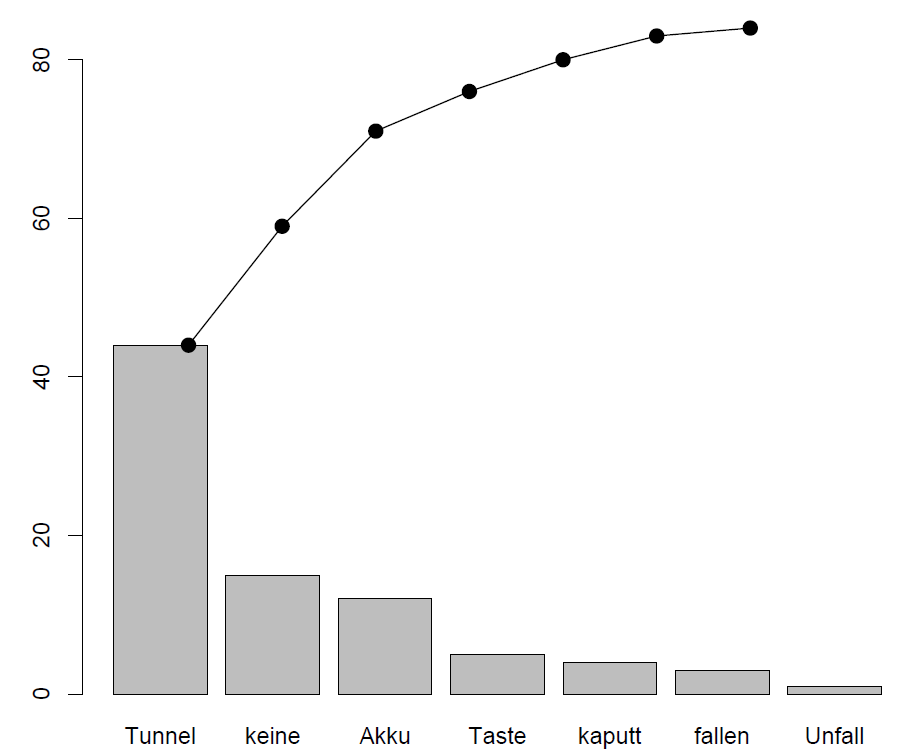
\includegraphics[width=0.3\linewidth]{figures/Pareto}
	\caption{Ein Pareto-Diagramm \textit{Quelle:}\cite{C:Pareto}}
	\label{fig:Pareto}
\end{figure}

\subsubsection{Ursache-Wirkungsdiagramm (Cause-and-Effect Diagramm)}
\label{subsubsec:UrsacheWirkungsDiagramm}
\begin{itemize}
	\item \glqq Fishbone-Diagramm\grqq 
	\item Grafische Strukturierung des Problems für übersichtliche Gesamtbetrachtung
	\item Der Kopf des Fisches stellt das Ziel dar
	\item Folgende Bereiche können gut als \glqq Top-Level-Fischgräte\grqq verwendet werden (jeweils inkl. Beispielen)
	\begin{itemize}
		\item Ausrüstung \textit{Software, Büroplatz, etc.}
		\item Umwelt \textit{Lärm, Hitze, etc.}
		\item Menschen \textit{Ausbildung, Motivation, etc.}
		\item Maschinen \textit{Bedienung, Alter, etc}
		\item Materialien \textit{Qualität, Beschaffung, etc.}
		\item Methoden \textit{Bestellung, Standartisierung, etc.}
	\end{itemize}
\end{itemize}

\subsection{Kontrollkarte}
\label{subsec:Kontrollkarte}
Die Grundlage einer Kontrollkarte bildet der statistische Test zur Prüfung einer statistischen Hypothese
\subsubsection{Basics}
\begin{itemize}
	\item $X$: Ein Zufallsvariabel
	\item $\mu_0$: Zielwert (gemäss Vorgabe, z.B. Fertigungszeichnung)
	\item $\mu_1$: Effektiver Mittelwert des gemessenen Parameters
	\item $\mu$: Wert des gemessenen Parameters
	\item $\delta_{1,2}$: Untere, resp. Obere Toleranzgrenze
	\item $\sigma^2$: Varianz
	\item $\sigma$: Standardabweichung
	\item $\bar{x}$: Aus Stichproben errechneter Mittelwert
	\item Standardfehler $=\frac{\sigma}{\sqrt{n}} = \sigma(\bar{X})$
	\item USL = Upper Specification Limit $\Rightarrow \mu_0+\delta_2$
	\item LSL = Lower Specification Limit $\Rightarrow \mu_0+\delta_1$
	\begin{itemize}
		\item Der durch UCL und LCL begrenzte Bereich heisst Kontrollbereich
	\end{itemize}
	\item $H_0$ Nullhypothese
	\begin{itemize}
		\item Annahme von $H_0$ Prozess ist unter Kontrolle (LCL $\leq \bar{x} \leq$ UCL)
	\end{itemize}
	\item Einem Test zu $n$ Zeitpunkten eine Serie von $m$ Proben entnehmen um die Zufallsvariabel $X$ zu bestimmen
	\begin{itemize}
		\item [$\rightarrow$] $n$ mal einen Versuch mit jeweils $m$ Proben (auf die gleiche Eigenschaft) geben $n$ Realisierungen der Variabel $X$
	\end{itemize}
	\item $z_q$: Quantil der Normalverteilung (siehe Tafel \ref{Anh:TafelqQuantileStandardisierteNormalverteilung}
	\begin{itemize}
		\item $\alpha$ Vorgegeben Irtumswahrscheinlichkeit $\in \left[0,0.5\right]$
		\item $z_q$ ist die Abweichung in $\sigma$ von $\mu_0$ 
		\item $P(Z\leq z_q =1-\frac{\alpha}{2}$ anhand von $\alpha$ das Zugehörige $q$ in Tabelle \ref{Anh:TafelqQuantileStandardisierteNormalverteilung} suchen
	\end{itemize}
	\item UCL und LCL entsprechend der Formel \ref{eq:UCLLCL1}  berechnen
	\begin{itemize}
		\item Mit dieser Formel berechnet sich aus der Streuung die zulässigen Toleranzbänder, damit ein gewisser Prozentsatz der Teile innerhalb dieses Bandes ist. 
	\end{itemize}
\end{itemize}
\begin{equation}
	\label{eq:UCLLCL1}
	\text{UCL} = \mu_0 + z_q\frac{\sigma}{\sqrt{n}} \qquad \text{und} \qquad
	\text{LCL} = \mu_0 - z_q\frac{\sigma}{\sqrt{n}}
\end{equation}

\subsubsection{Shewhart Kontrollkarte}
\begin{itemize}
	\item Da die Prozessstreuung meist unbekannt ist, muss diese aus einem Vorlauf geschätzt werden. 
	\item Die Karten werden in Paaren gebraucht (z.B. eine für Mittelwert, eine für Streuung)
	\item Ein Beispiel für die Datenaufnahem ist in Tabelle \ref{tab:RSKarte} gezeigt
	\begin{itemize}
		\item Es werden $k$ Stichproben gemacht (sog. Gruppen) mit jeweils $n$ Werten
	\end{itemize}
	\item Die Spannweite ist die Differenz zwischen minimalem und maximalen Wert einer Gruppe
	\item Die elementaren Formeln sind \ref{eq:Kontrollkarte1} und \ref{eq:Kontrollkarte2} gezeigt
\end{itemize}
\begin{table}[!h]
	\centering
	\begin{tabular}{c |c c c c cc|c|c|c}
		Stichprobe	& \multicolumn{6}{c|}{Stichprobenwert} & Mittelwert 	& Standardabweichung &Spannweite\\\hline
		1			&$x_{11}$&$x_{12}$&$\ldots$&$x_{1j}$&$\ldots$&$x_{1n}$&$\bar{x}_1$	&$s_1$	&$R_1$\\
		2			&$x_{21}$&$x_{22}$&$\ldots$&$x_{2j}$&$\ldots$&$x_{2n}$&$\bar{x}_2$	&$s_2$	&$R_2$\\
		$\vdots$	&$\vdots$&$\vdots$& 	   &$\vdots$&		 &$\vdots$&$\vdots$		&$\vdots$&$\vdots$\\
		i			&$x_{i1}$&$x_{i2}$&$\ldots$&$x_{ij}$&$\ldots$&$x_{in}$&$\bar{x}_i$	&$s_i$	&$R_i$\\
		$\vdots$	&$\vdots$&$\vdots$& 	   &$\vdots$&		 &$\vdots$&$\vdots$		&$\vdots$&$\vdots$\\
		k			&$x_{k1}$&$x_{k2}$&$\ldots$&$x_{kj}$&$\ldots$&$x_{kn}$&$\bar{x}_k$	&$s_k$	&$R_k$\\
	\end{tabular}
	\caption{Beispiel für $k$ Stichproben (Gruppen) mit jeweils $n$ Werten \textit{Quelle:}\cite{C:RSKarte}}
	\label{tab:RSKarte}
\end{table}
\begin{align}
	\label{eq:Kontrollkarte1}
	\bar{x}_i = \frac{1}{n}\sum_{j=1}^{n}x_{ij} \qquad \text{und} \qquad s_i=\sqrt{\frac{1}{n-1}\sum_{j=1}^{n}\left(x_{ij}-\bar{x}_i\right)^2}\\
	\label{eq:Kontrollkarte2}
	R_i = \max\left\lbrace x_{ij}\vert j\in \left\lbrace 1,\ldots,n\right\rbrace\right\rbrace - \min\left\lbrace x_{ij}\vert j\in \left\lbrace 1,\ldots,n\right\rbrace\right\rbrace
\end{align}

\subsubsection{$\bar{x}$ und $R$-Karte}
\begin{itemize}
	\item Für die Konstruktion der Karte werden $k$ Daten aus dem Vorlauf benutzt
	\item Die horizontale Achse der Karten ist jeweils der Index $i$, die vertikale Achse ist: 
	\begin{itemize}
		\item Spannweite bei der $R$-Karte
		\item Mittelwert bei der $\bar{x}$-Karte
	\end{itemize}
	\item Prozessstreuung zuerst unter Kontrolle bringen, danach die $\bar{x}$-Karte konstruieren
	\item Die Mittellinie (CL) der $R$-Karte wird mit $\bar{R}$ bezeichnet und berechnet sich gemäss Formel \ref{eq:xRKarte}
	\item Die Standardabweichung von $\bar{R}$ ist $\sigma_R$
	\item Wenn $\sigma_R$ normalverteilt ist, kann:
	\begin{itemize}
		\item für $\text{UCL}_R = D_4\bar{R}$ genommen werden
		\item für $\text{LCL}_R = D_3\bar{R}$ genommen werden
		\item $D_3$ und $D_4$ stammen von Anhang \ref{Anh:TafelFaktorenKontrollkarten} und hängen vom Stichprobenumfang $n$ ab
	\end{itemize}
	\item Vorgehen:
	\begin{itemize}
		\item [1.] Mittellinie, LCL und UCL in Karte eintragen
		\item [2.] Spannweiten $R_i$ eintragen im Streudiagramm eintragen
		\item Wenn Stichproben ausserhalb der Grenzen liegen, diese Messungen weglassen und Grenzen neu berechnen
	\end{itemize}
	\item Wenn $R$-Karte unter statistische Kontrolle ist, können für die Berechnung des UCL und des LCL auch die Formeln \ref{eq:xRKarte2} bis \ref{eq:xRKarte3} gebraucht werden
	\begin{itemize}
		\item Die Parameter $d_2$ und $A_2$ stammen aus Anhang \ref{Anh:TafelFaktorenKontrollkarten} und ist in Abhängigkeit der Anzahl Stichproben
		\item $\hat{\sigma}$ ist eine Schätzung für $\sigma$, siehe Formel \ref{eq:xRKarte4}
		\item $k^\ast$ bezeichnet Summe über alle gültigen Stichproben
	\end{itemize}
	\item Vorteil: Einfacher zu berechnen als $\bar{x}$-s-Karte
	\item \textbf{Formeln für die Berechnung von $\bar{x}$ und $R$-Karten}
\end{itemize}
\begin{align}
	\label{eq:xRKarte}
	\bar{R} &= \frac{1}{k}\sum_{i=1}^{k}R_i\\
	\label{eq:xRKarte4}
	\hat{\sigma} &= \frac{\bar{R}}{d_2}\\
	\label{eq:xRKarte2}
	\bar{\bar{x}} &= \frac{1}{k^\ast}\sum_{i=1}^{k^\ast}\bar{x}_i\\
	\label{eq:xRKarte3}
	\text{UCL}_{\bar{x}}  &= \bar{\bar{x}} + 3\frac{\bar{R}}{d_2\sqrt{n}} \approx \bar{\bar{x}}+A_2\bar{R} \qquad \text{und} \qquad \text{LCL}_{\bar{x}} = \bar{\bar{x}} - 3\frac{\bar{R}}{d_2\sqrt{n}} \approx \bar{\bar{x}}-A_2\bar{R}
\end{align}

\subsubsection{$\bar{x}$ und s-Karte}
\begin{itemize}
	\item Wie bei $\bar{x}$ und $R$-Karten zuerst die Streuung unter Kontrolle bringen
	\item Die horizontale Achse der Karten ist jeweils der Index $i$, die vertikale Achse ist: 
	\begin{itemize}
		\item Standardabweichung bei der $s$-Karte
		\item Mittelwert bei der $\bar{x}$-Karte
	\end{itemize}
	\item Parameter werden ebenfalls mit $k$ Stichproben aus einem Vorlauf berechnet
	\item Die Mittellinie ($\bar{s}$ ist das arithmetische Mittel aller Standardabweichungen des Vorlaufes
	\item UCL und LCL lassen sich mit $B_3$ und $B_4$ (aus Anhang \ref{Anh:TafelFaktorenKontrollkarten} berechnen
	\begin{itemize}
		\item $\text{UCL}_s = B_4\bar{s}$ und $\text{LCL}_s = B_3\bar{s}$
	\end{itemize}
	\item Vorteil der $\bar{x}$ und s-Karte: Nutzt vorhandene Informationen besser als $R$-$\bar{x}$-Karte
	\item \textbf{Formeln \ref{eq:xSKarte} bis \ref{eq:xSKarte3} für die Berechnung von $\bar{x}$ und $s$-Karten}
\end{itemize}
\begin{align}
	\label{eq:xSKarte}
	\bar{s} &= \frac{1}{k}\sum_{i=1}^{k}s_i\\
	\label{eq:xSKarte4}
	\hat{\sigma} &= \frac{\bar{s}}{c_4}\\
	\label{eq:xSKarte2}
	\bar{\bar{x}} &= \frac{1}{k^\ast}\sum_{i=1}^{k^\ast}\bar{x}_i\\
	\label{eq:xSKarte3}
	\text{UCL}_{\bar{x}} &= \bar{\bar{x}} + 3\frac{\bar{s}}{c_4\sqrt{n}} \approx \bar{\bar{x}}+A_3\bar{R} \qquad \text{und} \qquad \text{LCL}_{\bar{x}} = \bar{\bar{x}} - 3\frac{\bar{s}}{c_4\sqrt{n}} \approx \bar{\bar{x}}-A_4\bar{R}	
\end{align}

\subsubsection{Kontrollkarte für einzelne Messwerte}
\begin{itemize}
	\item Die horizontale Achse der Karten ist jeweils der Index $i$, die vertikale Achse ist: 
	\item Die vertikale Achse ist in der Einheit der gemessenen Grösse (z.b. \si{\milli\meter} und es werden gleich die gemessenen Grössen eingetragen
	\item Es gilt: Stichprobenumfang $n=1$
	\begin{itemize}
		\item Stichprobe besteht aus einer einzelnen Beobachtung
	\end{itemize} 
	\item Dies kann zur Anwendung kommen, wenn:
	\begin{itemize}
		\item Jedes produzierte Teil gemessen werden soll
		\item Die Produktion sehr viel Zeit in Anspruch nimmt
		\item Unterschied einer wiederholten Messung nicht auf die Prozessstreuung zurück zu führen ist. 
	\end{itemize}
	\item Die Kontrollkarte für einzelne Messwerte nutzt die gleitende Spannweite $\text{M}R_i$ zur Schätzung der Prozessstreuung 
	\item \textbf{Formeln \ref{eq:GleitendeSpannweite} bis \ref{eq:UCLLCLeinzelneMesswerte} für die Berechnung von Kontrollkarten für einzelne Messwerte}
\end{itemize}
\begin{align}
	\label{eq:GleitendeSpannweite}
	\text{M}R_i &=\left\lvert x_{i+1}-x_i \right\rvert\\
	\label{eq:MittelwertGleitendeSpannweite}
	\overline{\text{M}R} &= \frac{1}{n-1}\sum_{i=1}^{n-1}\text{M}R_i\\
	\label{eq:SchaetzungStreuung}
	\hat{\sigma} &= \frac{\overline{\text{M}R}}{d_2} = \frac{\overline{\text{M}R}}{1.128}\\
	\label{eq:UCLLCLeinzelneMesswerte}
	\text{UCL} &= \bar{x} + 3\frac{\overline{\text{M}R}}{1.128} \qquad \text{und} \qquad \text{LCL} = \bar{x} - 3\frac{\overline{\text{M}R}}{1.128}
\end{align}

\subsubsection{Die $P$-Kontrollkarte für relative Häufigkeiten}
\begin{itemize}
	\item Entgegen der anderen Kontrollkarten, wird für diese nur geprüft und nicht gemessen (entweder ist Anforderung erfüllt oder nicht)
	\item Somit braucht es Kontrollkarten für relative Häufigkeit 
	\item Benötigt grossen Stichprobenumfang
	\item $n$ der Stichprobenumfang in welchem wir $D$ defekte Teile finden
	\begin{itemize}
		\item $D$ ist binominalverteilt in $n$
		\item Verteilung hat unbekannte Erfolgswahrscheinlichkeit $p$
	\end{itemize}
	\item Relative Häufigkeit der Defekten Teile: Formel \ref{eq:RelHaeufigkeit}
	\item Varianz dieser Erfolgswahrscheinlichkeit Formel \ref{eq:VarianzRelHaeufigkeit}
	\item Die Erfolgswahrscheinlichkeit der $k$ einzelnen Stichproben als Formel \ref{eq:RelHaeufigkeitMultiple}
	\item Wenn alle $k^\ast$ gültigen Strichproben den gleichen Umfang haben:
	\begin{itemize}
		\item Formel \ref{eq:RelhaeufigkeitCL} für Mittellinie (Mittelwert der Wahrscheinlichkeiten)
		\item Formel \ref{eq:RelHaeufigUCLLCL} für die Kontrollgrenzen
	\end{itemize} 
	\item Wenn nicht alle $k^\ast$ Strichproben den gleichen Umfang haben:
	\begin{itemize}
		\item Formel \ref{eq:RelhaeufigkeitCL2} für Mittellinie (Mittelwert der Wahrscheinlichkeiten)
		\item Formel \ref{eq:RelHaeufigUCLLCL2} für die Kontrollgrenzen
		\item \textbf{Achtung:} Jetzt ist UCL und LCL von der Anzahl Proben abhängig und das Toleranzband muss nicht mehr unbedingt eine gerade Linie darstellen.
	\end{itemize} 
	\item Bei kleinen Stichprobenumfängen kann es sein, dass LCL negativ wird, in diesem Fall LCL=0 nehmen
	\item Vorteil: Günstig und einfach, Nachteil: Grosser Stichprobenumfang nötig
	\item \textbf{Formeln \ref{eq:RelHaeufigkeit} bis \ref{eq:RelHaeufigUCLLCL2} für die Berechnung von Kontrollkarten mit relativer Häufigkeit}
	\item $\hat{\sigma}$ kann geschätzt werden mit $\hat{\sigma}=\frac{\bar{s}}{c_4}$
	\begin{itemize}
		\item $c_4$ aus Anhang \ref{Anh:TafelFaktorenKontrollkarten}
	\end{itemize}
\end{itemize}
\begin{align}
	\label{eq:RelHaeufigkeit}
	\hat{p} &= \frac{D}{n}\\
	\label{eq:VarianzRelHaeufigkeit}
	\text{Var}\left(\hat{p}\right) &= \frac{p(1-p}{n}\\
	\label{eq:RelHaeufigkeitMultiple}
	p_1 &= \frac{d_1}{n_1},\ldots,p_k = \frac{d_k}{n_k}\\
	\label{eq:RelhaeufigkeitCL}
	\bar{p}&=\frac{1}{k^\ast}\sum_{i=1}^{k^\ast}p_i\\
	\label{eq:RelHaeufigUCLLCL}
	\text{UCL} &= \bar{p}+3\sqrt{\frac{\bar{p}(1-\bar{p}}{n}}		\qquad \text{und}\qquad
	\text{LCL} = \bar{p}-3\sqrt{\frac{\bar{p}(1-\bar{p}}{n}}\\
	\label{eq:RelhaeufigkeitCL2}	
	\bar{p}&= \frac{d_1+\cdots +d_{k^\ast}}{n_1+\cdots +n_{k^\ast}}\\
	\label{eq:RelHaeufigUCLLCL2}
	\text{UCL}_i &= \bar{p}+3\sqrt{\frac{\bar{p}(1-\bar{p}}{n_i}}		\qquad \text{und}\qquad
	\text{LCL}_i = \bar{p}-3\sqrt{\frac{\bar{p}(1-\bar{p}}{n_i}}\\
\end{align}
\clearpage
\subsection{Statistische Eigenschaften von Kontrollkarten}

\subsubsection{Interpretation von Kontrollkarten}
\begin{itemize}
	\item Zu jedem Zeitpunkt $t_i$ letzte $n_i$ der produzierten Teile entnehmen, messen, benötigte Werte berechnen und in Kontrollkarte eintragen
	\item Wenn der Prozess ausser Kontrolle ist (Punkte ausserhalb des Bereiches)
	\begin{itemize}
		\item [$\rightarrow$] Alle Teile zwischen letzter Messung und dieser Messung prüfen
		\item [$\rightarrow$] Fehler der Maschine korrigieren
		\item [$\rightarrow$] Prüfprozess beginnt wieder von vorne
	\end{itemize}
	\item Ermöglicht von Auge steigende oder fallende Tendenzen zu erkenne (indikation für systematischen Fehler)
	\item Ziel der Prozesskontrolle ist der Prozess unter statistischer Kontrolle zu halten
	\item \textbf{Western Electric Rules} zur Überwachung von Kontrollkarten, der Prozess ist ausser Kontrolle wenn:
	\begin{itemize}
		\item [1.] Ein Punkt ausserhalb von Bereich zwischen UCL und LCL liegt
		\item [2.] Zwei von drei aufeinanderfolgenden Punkten auf der gleichen Seite ausserhalb von $\frac{2}{3}$ des durch UCL und LCL festgelegten Bereich liegen ($\rightarrow$ Ausserhalb des 2-$\sigma$-Bereichs)
		\item [3.] Vier von fünf aufeinanderfolgenden Punkten auf der gleichen Seite ausserhalb von $\frac{1}{3}$ des durch UCL und LCL festgelegten Bereich liegen ($\rightarrow$ Ausserhalb des 1-$\sigma$-Bereichs)
		\item [4.] Acht aufeinanderfolgende Punkte auf der gleichen Seite der Mittellinie liegen
		\item Vorteil: Diese Regeln betrachten nicht nur einzelne Punkte sonder eine Abfolge und sucht ein Pattern
	\end{itemize}
\end{itemize}

\subsubsection{Fehler 1. und 2. Art}
\begin{itemize}
	\item \textbf{Fehler 1. Art}: richtige Nullhypothese wird abgelehnt (Detaillierte Erklärung: Skript s.29) 
	\begin{itemize}
		\item Es wird in Prozess eingegriffen obwohl dieser ungestört verläuft
		\item Wird als \textbf{blinder Alarm} bezeichnet
		\item Test der 0-Hypothese: $H_0:\mu=\mu_0$  
		\item Eine ungklücklich gewählte Stichprobe führt zum Prozesseingriff, obwohl dies nicht nötig wäre
	\end{itemize}
	\item \textbf{Fehler 2. Art}: falsche Nullyhpothese wird nicht abgelehnt
	\begin{itemize}
		\item Prozess läuft weiter, obwohl dieser derzeit gestört ist
		\item Wird als \textbf{unterlassener Alarm} bezeichnet
		\item Eine unglücklich erwischte Stichprobe führt dazu, dass Prozess weiter laufengelassen wird, obwohl dieser Fehlerhaft ist
	\end{itemize}
	\item Je kleiner $\alpha$ (Fehler 1. Art) gewählt wird, desto:
	\begin{itemize}
		\item Mehr geht die kritische Grösse $z_{1-\alpha}$ nach rechts
		\item desto kleiner wird das Risiko eine richtige Nullhypothese abzulehnen
		\item desto grösser wird $\beta$ (vom Fehler 2. Art) 
		\item desto grösser wird das Risiko für ein Fehler 2. Art
	\end{itemize}
	\item Eine Vergrösserung der Stichprobe kann obigen Problemen entgegenwirken. 
	\begin{itemize}
		\item Man spricht auch von einer Verbesserung der Trennschärfe
	\end{itemize}
	\item \textbf{Macht} Als Macht eines Tests wird die Wahrscheinlichkeit $1-\beta$ bezeichnet, mit der die Nullhypothese abgelehnt wird, wenn diese tatsächlich nicht stimmt
	\item  $\text{Macht} = P\left(\text{Entscheridung }H_0\text{nicht anzunhemen}\vert H_1 \text{sei richtig}\right)$
\end{itemize}

\subsubsection{Gütefunktion (und Eingriffsfunktion)}
\label{subsubsec:Guetefunktion}
\begin{itemize}
	\item Die Wahrscheinlichkeit die Nullhypothese $H_0$ abzulehnen, wenn $\mu_1$ vorliegt. 
	\begin{itemize}
		\item Mit anderen Worten: Den Fehler erkennen, wenn der Mittelwert $\mu_1$ abweicht vom eigentlichen Zielwert $\mu_0$
	\end{itemize}
	\item \textbf{Wahrscheinlichkeit eines unterlassenen Alarms:} $P(\delta) = 1-\tilde{g}(\delta)$
	\item Mit der normierten Variabel $\delta$ (Formel \ref{eq:delta}) messen der Abweichung vom gestörten zum ungestörten Prozess, in Einheiten von $\sigma$
	\item Gütefunktion hängt von $\mu_1$ und wird geschrieben: $g=g(\mu_1)$
	\item Wegen der Formel \ref{eq:delta} kann $g(\mu_1) = g(\delta\sigma+\mu_0) = \tilde{g}(\delta)$ festgelegt werden 
	\begin{itemize}
		\item Dabei ist $\delta$ eine Abweichung in $n\cdot\sigma$ von $\mu_0$ und $\sigma$ in der gleichen Einheit wie $\mu_0$ (z.B. \si{\milli\meter})
	\end{itemize}
	\item Die X-Achse der Gütefunktion ist in $\sigma$ und die Y-Achse ist gerade $\tilde{g}(\delta)$ 
	\item $\tilde{g}(\delta)$ wird als \textbf{Eingriffsfunktion} bezeichnet. 
	\begin{itemize}
		\item Für einen ungestörten Prozess (d.h. $\mu=\mu_0$ ) gilt $g(\mu_0) = \tilde{g}(0) = \alpha$
		\item $\alpha$ ist in Abhängigkeit vom erwarteten Signifikanzlevel (meist $\alpha = 0.0027$)
		\item Für einen gestörten Prozess sollte $g(\delta)$ möglichst gross sein
		\item Somit ist die Wahrscheinlichkeit für einen Unterlassenen Alarm ($P(\delta)=1-\tilde{g}(\delta)$) entsprechend klein
	\end{itemize}
	\item Formel \ref{eq:Phi} für die Berechnung der sich unter der Normalvertilung befindlichen Fläche
	\begin{itemize}
		\item Entspricht der Wahrscheinlichkeit ein Ergebnis in dieser Fläche zu treffen
		\item In Taschenrechner \glqq Menu $\rightarrow$ 5:Wahrscheinlichkeit $\rightarrow$ 5: Verteilungen $\rightarrow$ 2: Normal Cdf
		\item [] $\sigma$ ist dabei die Abweichung welche beim ersten $\sigma$ festzustellen ist
	\end{itemize}
	\item Operationscharakteristik: $\text{OC}(\mu_1)  = 1-g(\mu_1)$
	\begin{itemize}
		\item Stellt funktionalen Zusammenhang zwischen dem Fehler 2. Art und der Lage von $\mu_1$ her
		\item Wahrscheinlichkeit eines unterlassenen Alarmes, wenn $\mu_1$ vorliegt
	\end{itemize}
\end{itemize}
\begin{align}
	\label{eq:delta}
	\delta&=\frac{\mu_1-\mu_0}{\sigma}\qquad \Rightarrow \qquad \mu_1 = \delta\sigma+\mu_0\\
	\label{eq:Phi}
	\Phi(x,\mu,\sigma^2)&=\frac{1}{\sqrt{2\pi\sigma^2}}\int_{-\infty}^{x}e^{-\frac{\left( z-\mu\right)^2}{2\sigma^2}}\text{dz}
\end{align}

\subsubsection{Mittlere Lauflänge}
\label{subsubsec:MittlereLauflaenge}
\begin{itemize}
	\item Entgegen Kapitel \ref{subsubsec:Guetefunktion} interessieren wir uns nicht für die Wahrscheinlichkeit, dass ein Alarm bei einer einzelnen Stichprobe auftritt. Sondern wie lange es im Mittel dauert, bis wir in den Prozess eingreifen müssen. 
	\item Die Zeitspanne bis zu einem Eingriff wird \textbf{Lauflänge} resp \textbf{Run Length} genannt.
	\item Annahme Stichproben mit immer gleichem Umfang $n$ werden in regelmässige Abständen entnommen
	\begin{itemize}
		\item Wenn bei Stichprobe $i_{RL}$ erstmalig ein Eingriff nötig ist: Lauflänge ist $i_{RL}$
		\item Die Variabel $I_{RL}$ ist eine diskrete Zufallsvariabel mit der Wahrscheinlichkeit $p_k=P(I_{RL}=k)$ und $k\in\left\lbrace1,2,3,\ldots\right\rbrace$
	\end{itemize}
	\item Der Erwartungswert von $I_{RL}$ $\left( E\left(I_{RL}\right)\right)$ wird als \textbf{mittlere Lauflänge} resp. \textbf{Average Rung Lenght} bezeichnet, kurz \textbf{ARL}
	\begin{itemize}
		\item Diese beschreibt mittlere Zeitspanne bis Eingreifen in den laufenden Prozess nötig ist
		\item Hängt von Mittelwert $\mu_1$ und den Kontrollgrenzen ab
		\item Ein Prozess wäre ideal, wenn bei $\mu=\mu_0$ kein blinder Alarm auftritt (und somit kein Eingreifen nötig ist)
		\item Das Ereignis $I_{RL}=k$  tritt ein wenn der erste Eingriff bei der $k.$ Stichprobe erfolgt
		\item Mit Parameter $p$ (Formel \ref{eq:ParamP}) als Eingriffswahrscheinlichkeit (Wahrscheinlichkeit das Kontrollgrenze überschritten) haben wir:
		\begin{itemize}
			\item Wahrscheinlichkeit des Ereignises bei Stichprobe $k$ in Formel \ref{eq:geomverteilung}
			\item Der Erwartungswert der Variabel $I_{RL}$ in Formel \ref{eq:Erwartungswert}
		\end{itemize}
	\end{itemize}
	\item Für die mittlere Lauflänge folgt somit Formel \ref{eq:ARL2}. 
	\begin{itemize}
		\item Reminder: $\delta$ = Vielefaches für $\sigma$ gemäss Anforderungen an Prozess, 
		\item z.B. Wenn Irrtumswahrscheinlichkeit $\alpha = 0.0027$ ist, ist $\delta = 3$, siehe Anhang \ref{Anh:WichtigeSigma}
		\item Wenn ein ungestörter Prozess vorliegt ($\mu_1=\mu_0$, somit $\delta=0$) $\tilde{g}(0)=\alpha$
	\end{itemize}
\end{itemize}
\begin{align}
\label{eq:ARL}
\text{ARL} &= E\left(I_{RL}\right) = \sum_{k=1}^{\infty}kp_k\\
\label{eq:ParamP}
p &= p(\mu_1) = P(\mu\leq \text{LCL})+P(\text{UCL}\leq\mu) = g(\mu_1) = \tilde{g}(\delta)\\
\label{eq:geomverteilung}
p_k&= p(1-p)^{k-1}\\
\label{eq:Erwartungswert}
E(I_{RL}) &= \frac{1}{p}\\
\label{eq:ARL2}
\text{ARL}(\delta) &= \frac{1}{p(\mu)} = \frac{1}{g(\mu_1)}=\frac{1}{\tilde{g}(\delta)}
\end{align}

\subsubsection{Beispiel Guetefunktion und ARL}
\begin{figure}[!h]
	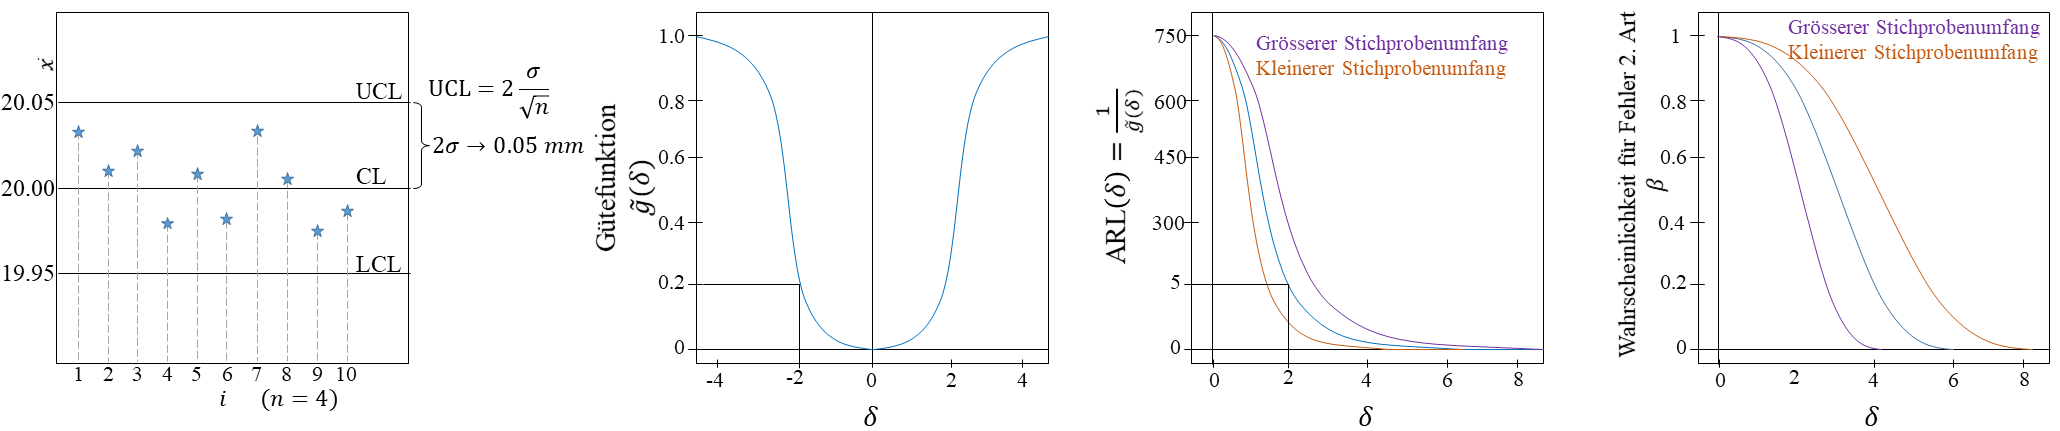
\includegraphics[width=1\linewidth]{figures/Guetefunktion3.png}
	%\caption{}
	\label{fig:guetefunktion}\\
	\begin{minipage}{1\linewidth}
		\begin{align*}
			\mu_0 &= \SI{20.000}{\milli\meter}\\
			\sigma &= \SI{0.05}{\milli\meter}\\
			n&=4\\
			\text{Irrtumswahrscheinlichkeit} &: \alpha = 0.0455\\
			\Rightarrow  & 2\sigma \text{ Aus Tabelle in Anhang \ref{Anh:WichtigeSigma}}\\
			\text{UCL/LCL}&: \mu_0\pm 0.05\\
			\sigma = 2\sigma &\rightarrow \delta=2\\ 
			\Rightarrow \tilde{g}(\delta) &= \tilde{g}(2)=0.2\\ 
			\Rightarrow \text{ARL}(2) &= 5 
		\end{align*}
	Benötigte Werte in Abh. $\delta$ aus Diagrammen lesen
	\end{minipage}
\end{figure}

\subsubsection{Prozessfähigkeit}
\begin{itemize}
	\item \textbf{Prozessbereich}: Wenn zulässiger Bereich $\left[\mu_0-3\sigma, \mu_0+3\sigma\right]$ ist, ist Prozessbereich $6\sigma$
	\begin{itemize}
		\item Achtung:Kontrollgrenzen (UCL und LCL) sind abhängig von Stichprobenumfang und nicht somit nur bei $n=1$ identisch mit Prozessbereich
	\end{itemize}
	\item \textbf{Toleranzgrenzen} USL und LSL sind bei Fertigung einzuhalten
	\item Die \textbf{Toleranzmitte} (SL) Mittelwert Zwischen oberer und unterer Toleranzgrenze
	\item Der \textbf{Prozessfähigkeitsindex} (PCR) drückt Verhältnis zwischen Breite des Toleranzbereiches und Breite des Prozessbereiches aus
	\item Unter der Annahme, dass Prozess unter Kontrolle ist ($\mu_1 = \mu_0$ und SL$=\mu_0$) gilt:
	\begin{itemize}
		\item PCR $= 1 \rightarrow$ Ausschussquote von genau $\alpha$ liegt vor
		\item PCR $< 1 \rightarrow$ Ausschussquote von mehr als $\alpha$ liegt vor. Prozessfähigkeit nicht vorhanden
		\item PCR $> 1 \rightarrow$ Ausschussquote von weniger als $\alpha$ liegt vor. Prozessfähigkeit vorhanden
	\end{itemize}
	\item Achtung: Wenn Zielwert $\mu_0$ und Prozessstreuung $\sigma$ nicht bekannt ist (der Normalfall), reagieren diese Schätzungen sehr empfindlich auf, wenn Prozess nicht unter Kontrolle ist, oder keine Normalverteilung der Messgrösse vorliegt
\end{itemize}
\begin{align}
	\text{SL} &= \frac{\text{USL}+\text{LSL}}{2}\\
	\text{PCR} &= C_p = \frac{\text{USL}-\text{LSL}}{6\sigma} \qquad \text{Achtung: 6 hängt ab von gegebner Irrtumswahrscheinlichkeit }\alpha \text{, hier }\alpha=0.0027\\
\end{align}

\newpage


\subsection{Kontrollkarten mit Gedächnis}
\begin{itemize}
	\item Bei klassischen (Shewart) Kontrollkarten erfolgt Entscheid über Eingriff auf Basis des Ergebnisses einer Stichprobe
	\begin{itemize}
		\item Vergangenheit wird nicht mitberücksichtigt
	\end{itemize}
	\item Wird die Vergangenheit mit Berücksichtigt ist es eine \textbf{Kontrollkarte mit Gedächtnis}
	\item Vorteil: Störungen können schneller aufgedeckt werden
	\item Kontrollkarten mit Gedächtnis basieren auf Linearkombination einiger (oder aller)  vor Zeitpunkt $i$vorgenommenen Stichproben
	\item Die allgemeine Formel dafür ist Formel \ref{eq:gedaechtnisAlg}
	\item Die Parameter $\alpha_i$ und $\beta_i$ legen den Typ der Kontrollkarte fest
	\begin{itemize}
		\item Wenn z.B $\alpha_i = 0$ , $\beta_1\ldots\beta_{i-1} = 0$ und $\beta_i=1$ ist das die gedächtnislose Shewart $\bar{x}$-Karte
	\end{itemize}
	\item Je kleiner $\left\vert \delta\right\rvert$ ist (siehe Formel \ref{eq:delta}), desto rascher wird eine Abweichung vom Zielwert ($\mu_0$) erkannt.
	\begin{itemize}
		\item Desto kürzer ist die ARL (mittlere Lauflänge, Kapitel \ref{subsubsec:MittlereLauflaenge})
	\end{itemize}
\end{itemize}
\begin{align}
	\label{eq:gedaechtnisAlg}
	y_i&= \alpha_i + \sum_{j=1}^{i}\beta_j\bar{x}_i
\end{align}

\subsubsection{CUMSUM}
\begin{itemize}
	\item Cumulative Sum Control Chart, Karte zur Kontrolle der Mittelwerte
	\item Trägt die Kummulative Abweichung der Stichproben zu dem Zielwert auf, sofern diese eine gewisse Grenze überschreiten
	\item Kann sowohl für einzlene Beobachtungen, wie auch für Stichproben verwendet werden
	\item Für Prozesse Empfohlen bei denen bereits kleine Störungen bedeutsam sind und aufgedeckt werden müssen
	\item CUMSUM-Karte verwendet zwei \glqq Speicherwerte\grqq für Aufsummieren der Abweichung
	\begin{itemize}
		\item Formel \ref{eq:CUMSUMPlus} für obere Grenze und Formel \ref{eq:CUMSUMPlus} für untere Grenze
		\item Beide dieser Werte müssen mit jedem neuen Messwert aktualisiert werden
		\item $K$ ist hierbei der Referenzwert, es werden nur Fehler erkannt, die diesen Überwiegen
		\item Ein guter Wert für $K$: siehe Formel \ref{eq:CUMSUMK}
		\item Soll ein Shift von $\Delta$ aufgedeckt werden $\Rightarrow K =\frac{\Delta}{2}$ 
		\item Es werden also nur Werte Berücksichtigt die einen Abstand $>K$ von $\mu_0$ haben
	\end{itemize}
	\item Der Prozess ist unter Kontrolle, wenn der Erwartungswert von $E(C_i^+)=E(C_i^-)=0$ ist
	\item Der Prozess ist ab einem gewissen Index $i_0$ ausser Kontrolle wenn einer Erwartungswert eine Konstante $H$ überschreitet
	\begin{itemize}
		\item Den Prozess stoppen und in Ordnung bringen, Anschliessend neustarten und $C_i^+ = C_i^- = 0$ setzten
		\item $H$ wird auch \textbf{Entscheidungsintervall} genannt
		\item Ein guter Wert für $H$ ist in Formel \ref{eq:CUMSUMK} gezeigt (wenn zulässiger Bereich $\pm 3\sigma$ ist)
	\end{itemize}
\end{itemize}
\begin{align}
	\label{eq:CUMSUMPlus}
	C_i^+&=\max\left\lbrace 0,\bar{x}_i-(\mu_0+K)+C_{i-1}^+\right\rbrace\\
	\label{eq:CUMSUMMinus}
	C_i^-&=\max\left\lbrace 0,(\mu_0-K)-\bar{x}_i+C_{i-1}^-\right\rbrace\\
	\label{eq:CUMSUMK}
	K &= \frac{\hat{\sigma}}{2}\qquad \text{und}\qquad H=5\hat{\sigma}
\end{align}

\subsubsection{EMWA}
\begin{itemize}
	\item \textbf{Exponentially Weighted Movin Average} Karte zur Mittelwertskontrolle
	\item Gewicht $\beta$ in Formel \ref{eq:gedaechtnisAlg} klingt expontentiell ab (mit dem zuhnemenden \glqq Alter \grqq der jeweiligen Stichprobe)
	\item Der Glättungsfaktor $\lambda$ bestimmt den Einfluss der zurückliegenden Stichprobenmittelwerte $\bar{x}_j$
	\begin{itemize}
		\item Je kleiner $\lambda$ dest mehr Werte $\bar{x}_j$ werden zur Entscheidung herangezogen (langes Gedächtnis)
		\item Die Grenzen UCL$_i$ und LCL$_i$ steigen bei grösserem $\lambda$ schneller an
		\item EMWA-Karte hat somit ein ungleichmässiges, unbegrenztes Gedächtnis
		\item Für $\lambda=1$ haben wir die Shewhart $\bar{x}$-Karte
	\end{itemize}
	\item Den Wert $y_i$ zum $i.$ Zeitpunkt kann gemäss Formel \ref{eq:EWMAalg} absolut berechnet werden oder mit Formel \ref{eq:EWMArek} rekursiv
	\item Die Kontrollgrenzen berechnen sich gemäss Formel \ref{eq:EWMAkontrollgrenze}
	\begin{itemize}
		\item \textbf{Achtung}: Diese ist Abhängig von der Messnummer $i$ und ändert sich somit mit jeder Messung 
		\item Änderung zu beginn stark, anschliessend immer weniger, Funktion sieht aus wie Schrittantwort von PT1-Glied
		\item Bereits für Mittelgrosse $i$ ist die Funktion asymptotisch und es ergeben sich die von $i$ unabhängigen Grenezn in Formel \ref{eq:EWMAkontrollgrenzeinf}
	\end{itemize}
\end{itemize}
\begin{align}
	\label{eq:EWMAalg}
	y_i &= \underbrace{(1-\lambda)^{i}\mu_0}_{\alpha_i}+\sum_{j=1}^{i}\underbrace{(1-\lambda^{i-j})}_{\beta_i}\bar{x}_j\\
	\label{eq:EWMArek}
	y_i&=(1-\lambda)y_{i-1}+\lambda\bar{x}_i\\
	\label{eq:EWMAkontrollgrenze}
	\text{UCL}_i &= \mu_0 + 3\frac{\sigma}{\sqrt{n}}\sqrt{\frac{\lambda}{2-\lambda}(1-(1-\lambda)^{2i})}	\quad &\text{und} \qquad
	\text{LCL}_i &= \mu_0 - 3\frac{\sigma}{\sqrt{n}}\sqrt{\frac{\lambda}{2-\lambda}(1-(1-\lambda)^{2i})}\\
	\label{eq:EWMAkontrollgrenzeinf}
	\text{UCL} &= \mu_0 + 3\frac{\sigma}{\sqrt{n}}\sqrt{\frac{\lambda}{2-\lambda}} 	\quad &\text{und} \qquad
	\text{LCL} &= \mu_0 - 3\frac{\sigma}{\sqrt{n}}\sqrt{\frac{\lambda}{2-\lambda}}
\end{align}

\subsection{Annahmekontrolle, Zählende Prüfung}
\begin{itemize}
	\item Aufgrund von Informationen aus einer Stichprobe entscheiden über die Qualität des ganzen Loses
	\item Mittelweg zwischen keiner Kontrolle und 100\%-Kontrolle
	\item Basierend auf Prüfplänen
	\item Kann im gegensatz zu vorherigen Prüfungen nicht in Prozess eingreifen
	\item \textbf{Los} Menge eines Produktes das unter gleichen Bedingungen entstanden ist und als einheitlich angesehen werden kann
\end{itemize}

\subsubsection{Prüfpläne für Zählende Prüfung}
\begin{itemize}
	\item $N$ Einheiten hat ein Los
	\item $m$ Einheiten eines Loses sind ausschuss
	\item $p$ Ausschussquote $p=\frac{m}{N}$, Problem dabei ist, dass $m$ nicht bekannt ist
	\item $n$ Stichprobenumfang
	\item $x$ eine Regel (z.B. für eine Eigenschaft)
	\item $c$ Annahmezahl, solange weniger Ausschuss in einem Los enthalten ist wieder dieses angenommen
	\begin{itemize}
		\item $x<\leq c$ Los wird angenommen, andernfalls abgelehnt
	\end{itemize}
	\item $n$ und $c$ sind die \textbf{Kenngrössen} eines Prüfplans
	\item $H_0$: $x\leq c$ d.h. das Los wird angenommen
	\item $\alpha$ Produzentenrisiko (siehe Kaptiel \ref{subsubsec:Fehler})
	\item $\beta$ Konsumentenrisiko (siehe Kaptiel \ref{subsubsec:Fehler})
\end{itemize}

\subsubsection{Fehler 1. Art und 2. Art}
\label{subsubsec:Fehler}
\begin{itemize}
	\item \textbf{Fehler 1. Art} liegen vor, wenn ein eigentlich gutes Los wegen einer schlechten Stichprobe retourniert
	\begin{itemize}
		\item Bezeichnet als das Produzentenrisiko
		\item Wird mit $\alpha$ bezeichnet
	\end{itemize}
	\item \textbf{Fehler 2. Art} liegen vor, wenn ein eigentlich schlechtes Los wegen einer gut scheinenden Stichprobe angenommen wird
	\begin{itemize}
		\item Bezeicht als Konsumentenrisiko
		\item Wird mit $\beta$ bezeichnet
	\end{itemize}
	\item Vom Produzent festgelegte Grenze für Retournierung: $p_\alpha$ $\rightarrow$ annehmbare Qualitätslage
	\item Vom Konsument festgelegte Grenze für Retournierung: $p_\beta$ $\rightarrow$ rückweisende Qualitätslage
	\begin{itemize}
		\item Es muss $p_\alpha<p_\beta$ gelten
		\item Der Produzent will wenn möglich Lose mit $p<p_\alpha$ nicht zurücknehmen
		\item Der Konsument will wenn möglich Lose mit $p_\beta<p$ nicht annehmen
	\end{itemize}
	\item Ein Prüfplan minimiert $\alpha$ und $\beta$ möglichst fest, d.h. es werden möglichst keine Fehlentscheide getroffen
\end{itemize}

\subsubsection{Operationscharakteristik}
\begin{itemize}
	\item Die Operationscharakteristik eines Prüfplans stellt einen Zusammenhang zwischen den vier Grössen ($\alpha, \beta, p_\alpha \text{ und } p_\beta$) her
	\item Beschreibt die Annahmewahrscheinlichkeit eines Loses in Abhängigkeit der Ausschussquote $p$
	\item $\text{OC:} \left[0,1\right]\rightarrow \left[0,1\right]$
	\item Je grösser die Ausschussquote $p$ ist, desto kleiner soll die Annahmewahrscheinlichkeit (OC) sein
	\begin{itemize}
		\item Für $p=0$ soll $\text{OC}=1$ sein $\Rightarrow \text{OC}(0)=1$ (Lieferung wird sicher angenommen)
		\item Für $p=1$ soll $\text{OC}=0$ sein $\Rightarrow \text{OC}(1)=0$ (Lieferung wird sicher abgelehnt resp. retourniert)
	\end{itemize}
	\item $p^\ast$ ist die Zulässige Ausschussquote, mit dieser lässt sich OC gemäss der Gleichung \ref{eq:OC} ausdrücken
	\begin{itemize}
		\item Eine Vollständige Prüfung ist in der Regel nicht möglich, daher wird folgendes definiert
		\item Anzahl $x$ defekter Einheiten ist höchsten gleich Annahmezahl $c$
		\item Es liegen also $N$ Einheiten vor, mit $m (=pN)$ schlechten und somit mit $N-m (=N-pN)$ guten Einheiten, davon wird eine Stichprobe $n$ gezogen. Die Wahrscheinlichkeit, dass sich unter den $n$ einheiten höchsten $c$ Einheiten Ausschuss befinden ist in Formel \ref{eq:OCp} berechnet. Annahme resp. Ablehnung bestimmen mit Gleichung \ref{eq:OC}
		\item Die Anzahl defekter Einheiten ist X, es handelt sich dabei um eine hypergeometrische Zufallsvariabel
	\end{itemize}
	\item Für Visualisierungen der OC siehe Skript s. 56
	\item Zusammenhang zwischen Fehler der 1.- und 2. Art ist gegeben wie folgt:
	\begin{itemize}
		\item $\text{OC}(p_\alpha) = 1-\alpha$
		\item $\text{OC}(p_\beta) = \beta$
	\end{itemize}
\end{itemize}
\subsubsection{Kenngrössen eines Prüfplanes bestimmen}
\begin{itemize}
	\item Vorraussetzung Produzent und Konsument sind sich einig über $\alpha, \beta, p_\alpha \text{ und } p_\beta$
	\begin{itemize}
		\item Somit sind zwei Punkte der OC-Kennlinie (nämlich $(p_\alpha,1-\alpha) \text{ und } (p_\beta,\beta)$ gegeben
	\end{itemize}
	\item Zu bestimmen ist $n$ (Stichprobenumfang) und $c$ (Annahmezahl)
\end{itemize}

\begin{align}
	\label{eq:OC}
	\text{OC}(p) &= \left\lbrace \begin{matrix}
		1 & \qquad &\text{wenn } &p\leq p^\ast \qquad &\Rightarrow &\text{Annahemen}\\
		0 & \qquad &\text{wenn } &p^\ast> p 	\qquad &\Rightarrow &\text{Ablehnen}
	\end{matrix}\right.\\
	\label{eq:OCp}
	\text{OC}(p) &= P(X\leq c) = \sum_{k=0}^{c}P(X=k) = \sum_{k=0}^{c}\frac{\binom{pN}{k}\binom{N-pN}{n-k}}{\binom{N}{n}}
\end{align}

\clearpage
\section{Regressionsrechnung}
\subsection{Lineare Regression}
\begin{itemize}
	\item Statistische Methode zum Untersuchen und Modellieren der Zusammenhänge zwischen (Mess-)Grössen
	\item $y_i$ ist eine Beobachtung 
	\item $x^{(1)},x^{(2)},\ldots,x^{(m)}$ oder $x_1,x_2,\ldots,x_m$ sind erklärende Variablen 
	\item $y_i$ hängt über eine Funktion $h$ mit den Variablen $x^{(1)},x^{(2)},\ldots,x^{(m)}$ zusammen
	\item Ziel ist des die Funktion $h$ zu finden, sodass diese für jedes $y_i$ gilt
	\begin{itemize}
		\item Eine solche Formel existiert nicht, da es jeweils Abweichungen gibt, also muss sie lauten:
		\item $y_i = h\left(x^{(1)},x^{(2)},\ldots,x^{(m)}\right)+E_i$
	\end{itemize}
	\item $E_i$ ist also der Zufallsfehler (kann von unterschiedlichen Bedingungen, Messungenauigkeiten, etc. abhängige)
	\begin{itemize}
		\item Dieser Fehler muss sich als Wahrscheinlichkeitsverteilung vorgestellt werden
		\item [$\rightarrow$] Normalverteilung mit Erwartungswert 0 und Varianz $\sigma^2 \rightarrow\mathcal{N}(0,\sigma^2)$ 
	\end{itemize}
\end{itemize}
\subsubsection{Transformationen}
\begin{itemize}
	\item Datentransformation kann sinnvoll sein, z.B. Logarithmieren
	\begin{itemize}
		\item So kann $y = C\cdot \frac{x_1}{x_2^2}$ Logarithmiert zu $\log(y) = \log(C)+\log(x_1)-2\cdot\log(x_2)$
	\end{itemize}
\end{itemize}

\subsubsection{Schätzung der Parameter}
\begin{itemize}
	\item Schätzen nach dem Prinzip der kleinsten Quadrate
	\begin{itemize}
		\item Die Summe aller $r_i^2$ soll minimiert werden, siehe Abbildung \ref{fig:reg1}
		\item Die Formel \ref{eq:Reg1} und \ref{eq:Reg2} zeigt die Bestimmung von den Schätzwerten $\hat{\alpha}$ und $\hat{beta}$ 
		\item Dabei ist $\bar{x}$ der Mittelwert aller $x$, dasselbe für $\bar{Y}$
		\item Die Regression berechnet sich aus $n$ Messpunkten
	\end{itemize}
	\item Die geschätzten Parameter $\hat{\alpha}$ und $\hat{\beta}$  treten ebenfalls in der Normalverteilung um ihren Erwartungswert auf
	\begin{itemize}
		\item Somit ist $\hat{\beta}\sim\mathcal{N}\left(\beta,\sigma^{(\beta)2}\right)$ und $\hat{\alpha}\sim\mathcal{N}\left(\alpha,\sigma^{(\alpha)2}\right)$	
	\end{itemize}
\end{itemize}
\begin{figure}[h!]
	\begin{minipage}{0.4\linewidth}
		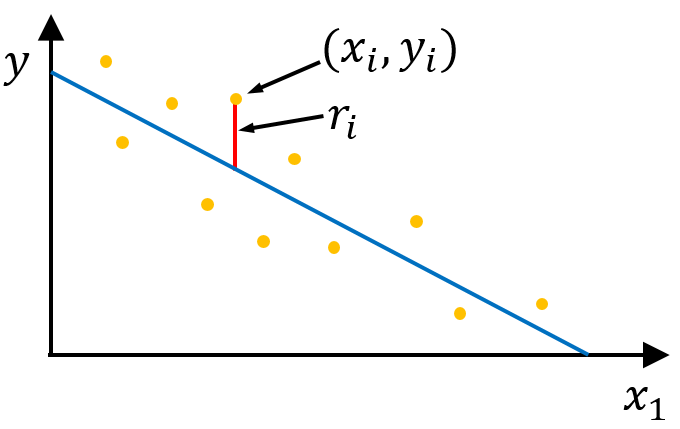
\includegraphics[width=0.8\linewidth]{figures/Reg1}
		\caption{Lineare Regression mit eingezeichnetem Fehler}
		\label{fig:reg1}
	\end{minipage}
	\begin{minipage}{0.7\linewidth}
		\begin{align}
			\label{eq:Reg1}
			\hat{\beta}&=\frac{\sum_{i=1}^{n}\left(\left(Y_i-\bar{Y}\right)\left(x_i-\bar{x}\right)\right)}{\sum_{i=1}^{n}\left(x_i-\bar{x}\right)^2}\\
			\label{eq:Reg2}
			\hat{\alpha}&= \bar{Y}-\hat{\beta}\bar{x}\\
			\label{eq:RegVarianz}
			\hat{\sigma}^2&=\frac{1}{n-2}\sum_{i=1}^{n}R_i^2\\
			\hat{y} &= \hat{\alpha}+\hat{\beta}x
		\end{align}
	\end{minipage}
\end{figure}

\subsubsection{Residuen und Varianzeinschätzung}
\begin{itemize}
	\item Zufällige Fehler $E_i$ können nicht beobachtet werden
	\item Bekannt sind die Näherungswerte für $E_i$ diese heissen \textbf{Residuen}
	\item Fehler Streuen mit Varianz $\text{var}(E_i) = \sigma^2$
	\item Die Schätzung für die Varianz ist in Formel \ref{eq:RegVarianz} gezeigt (neben Abbildung \ref{fig:reg1})
\end{itemize}

\subsubsection{Tests und Vertrauensinterval}
\begin{itemize}
	\item Frage nach möglicher Abweichung zwischen den geschätzten Parametern (z.B. $\hat{\beta}$) und den effektiven Parametern (z.B. $\beta$)
	\item Sind die Daten mit einem Modell  mit (teilweise) vorgegebenen Parametern verträglich?
	\item Definieren einer Nullhypothese, z.B. $H_0: \beta = -2$ wird anschliessend oft mit $\beta^0$ bezeichnet
	\item Gemäss den Formeln \ref{eq:regH0} und \ref{eq:regH01} den T-Wert bestimmen
	\item Diesen Wert T-Wert mit dem T-Wert des festgelegten Niveaus vergleichen (meist 5\%)
	\begin{itemize}
		\item Der Wert des festgelegten Niveau ist in Anh. \ref{Anh:TafelStudentTVerteilung} zu finden
		\item Für 5\%-Niveau die Spalte 0.9750 betrachten!
		\item In Abhängigkeit der Anzahl Datenpunkte
	\end{itemize}
	\item Wenn der berechnete T-Wert kleiner ist als jener der Tabelle: 
	\begin{itemize}
		\item Die Nullhypothese für den gewählten Wert (z.B. $\beta=2$) kann \textbf{nicht} abgelehnt werden
	\end{itemize}
	\item \textbf{Das Vertrauensintervall umfasst alle Punkte deren $H_0$ nicht abgelehnt werden kann}
\end{itemize}
\begin{align}
	\label{eq:regH0}
	T&= \frac{\hat{\beta}-\beta^0}{\text{se}(\hat{\beta})} \qquad \text{mit} \qquad \text{se}(\hat{\beta})=\sqrt{\frac{\sigma^2}{\text{SS}_x}}\\
	\label{eq:regH01}
	\text{SS}_x &= \sum_{i=1}^{n}(x_i-\bar{x})^2
\end{align}

\subsubsection{Vertrauens- und Prognosebereich}
\label{subsubsec:VertrauensUndPrognoseBereich}
\begin{itemize}
	\item Der Vertrauensbereich wird auch als Konfidenzintervall bezeichnet
	\item Oftmals wird hier wieder das 95\%-Vertrauensintervall verwendet 
	\item Die Formeln für die Berechnung des Vertrauensintervall ist \ref{eq:Vertrauensintervall} (für $SS_x$ siehe Formel \ref{eq:regH01}
	\begin{itemize}
		\item der Wert $c_w$ stammt ebenfalls aus Anhang \ref{Anh:TafelStudentTVerteilung}, für 95\% Vertrauensintervall Wert von Spalte 0.975 nehmen, für $n-2$ Freiheitsgrade
		\item Mit dieser Formel erhalten wir die Punkte des Vertrauensintervall oben- und unten an $h(x_0)$ 
		\item Alle plausiblen Werte $\eta$ liegen in diesem Vertrauensbereich und erfüllen somit die Nullhypothese $\eta_0 = \eta_0^o$
	\end{itemize}
	\item Das Vertrauensintervall erklärt nicht in welchem Bereich künftige Beobachtungen zu erwarten sind!
	\item Das Prognoseintervall berücksichtigt zusätzlich noch die Variabilität von $E_i$
	\begin{itemize}
		\item Das Prognoseintervall für die 95\%-Grenze kann gemäss Formel \ref{eq:Prgronoseintervall} berechnet werden
		\item $c_w$ Wert wie zuvor aus Anhang \ref{Anh:TafelStudentTVerteilung}, ebenfalls wieder bei $n-2$ Messungen schauen!
	\end{itemize}
	\item Abbildung \ref{fig:ProgrnoseUndVertrauen} Verdeutlicht das Aussehen dieser zwei Bänder
\end{itemize}
\begin{align}
	\label{eq:Vertrauensintervall}
	\text{Vertrauensintervall} &= \hat{\eta}_\pm c_w \cdot \text{se}\left(\hat{\eta}_0\right) \qquad= \left(\hat{\alpha}+\hat{\beta}x_0\right)\pm c_w \cdot \text{se}\left(\hat{\eta}_0\right) \qquad
	\text{se}\left(\hat{\eta}_0\right) = \hat{\sigma}\sqrt{\frac{1}{n}+\frac{(x_0-\bar{x})^2}{SS_x}}\\
	\label{eq:Prgronoseintervall} 
	\text{Progrnoseintervall} &= \hat{\eta}_0\pm c_w \cdot \sqrt{\hat{\sigma}^2+\left(\text{se}^2\left(\hat{\eta}_0\right)\right)} \qquad= \left(\hat{\alpha}+\hat{\beta}x_0\right)\pm c_w \cdot \sqrt{\hat{\sigma}^2+\left(\text{se}^2\left(\hat{\eta}_0\right)\right)}
\end{align}
\begin{figure}[!h]
	\centering
	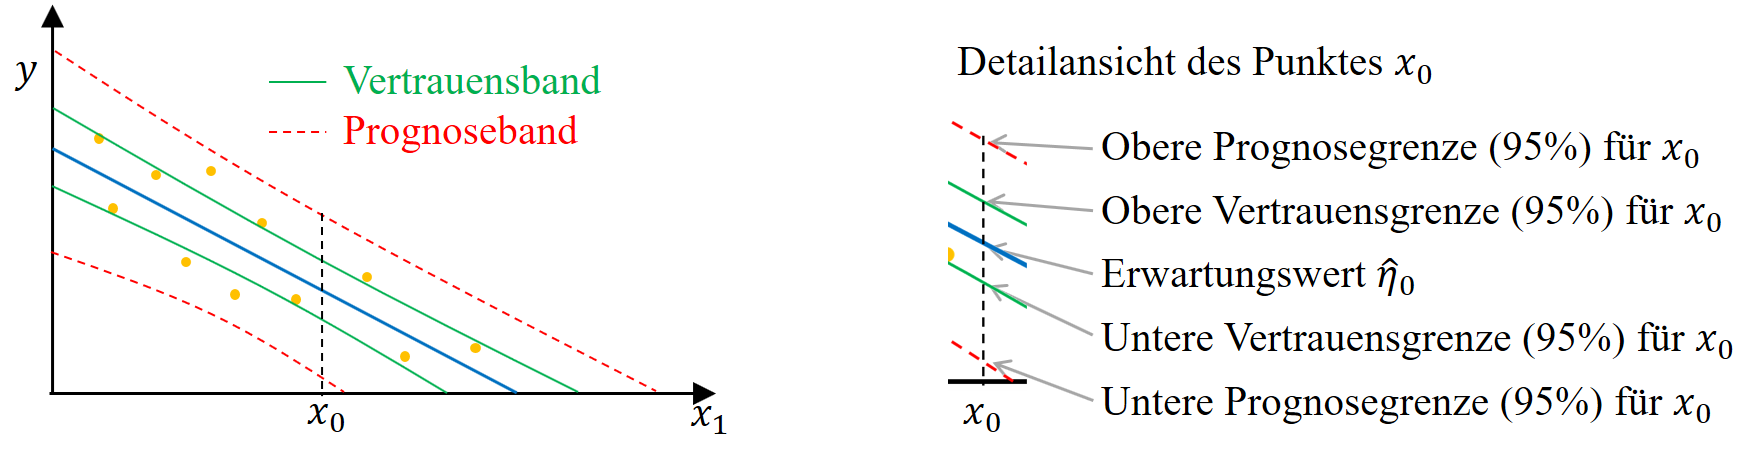
\includegraphics[width=0.7\linewidth]{figures/ProgrnoseUndVertrauensband}
	\caption{Prognose- und Vertrauensband}
	\label{fig:ProgrnoseUndVertrauen}
\end{figure}

\subsection{Prüfen der Modelleignung}
\label{subsec:PruefenModelleignung}
Die Problemstellung ist, dass gewisse Annahmen gemacht werden müssen. Dabei ist die zentrale Annahme, dass die Fehler $E_i$ unabhängig und normalverteilt sind mit konstanter Varianz. $\rightarrow E_i \sim \mathcal{N}\left(0,\sigma^2\right)$  Diese Annahme kann aufgespalten werden in:
\begin{itemize}
	\item Der Erwartungswert $E_i$ ist $E(E_i)=0$
	\begin{itemize}
		\item Punkte Streuen Symmetrisch um lineare Regression
	\end{itemize}
	\item Die $E_i$ haben alle die gleiche Varianz $\text{var}(E_i)=\sigma^2$
	\begin{itemize}
		\item Über die ganze Länge d haben die gemessenen Punkte ($y_i$) in etwa den gleichen Abstand linearen Regressionsgeraden
	\end{itemize}
	\item $E_i$ ist Normalverteilt ($\rightarrow$ Glockenkurve, wenn deren Häufigkeit aufgetragen würde)
	\item $E_i$ sind unabhängig
\end{itemize}

\subsubsection{$R^2$ Bestimmtheitsmass}
\label{subsubsec:R2Bestimmtheitsmass}
Güte der Anpassung der Linearen Regression bestimmen
\begin{itemize}
	\item $R^2\in\left[0,1\right]$ und misst Anteil der durch die Regression erklärte Streung des Y-Wertes 
	\item Quantifiziert den linearen Zusammenhang zwischen den angepassten Werten und den Beobachtungen (quadrierte Korrelation zwischen den Werten)
	\item Je \textbf{grösser} $R^2$ ist, desto \textbf{besser}
	\item Formel \ref{eq:RSquare} Für Berechnung von $R^2$
	\item Quadrat der Summen aller (mit $\alpha$ und $\beta$) geschätzten y-Werte ($\hat{y}$ an den Stellen wo wir ein $y$ haben, dividiert durch das Quadrat der Summe aller gemessenen $y_i$
	\item \textbf{Achtung:} Bestimmtheitsmass gibt keine Auskunft über Eignung des Modells
	\item Das Regressionsmodell erfasst $R^2\cdot 100\%$ der Variabilität in den Zielvariablen
\end{itemize}

\begin{align}
\label{eq:RSquare}
R^2 &= \frac{\sum_{i=1}^{n}\left(\hat{y}_i-\bar{\hat{y}}\right)^2}{\sum_{i=1}^{n}\left(y_i-\bar{y}\right)^2}
\end{align}


\subsubsection{Diagnose Instrumente}
\begin{itemize}
	\item Schwankungen der erwähnte Abweichung (Residuum) zwischen der geschätzten Regressionsgeraden und den gemessenen Punkten  ist von Auge nur schwer zu erkennen
	\item Besser erkennbar wird diese, wenn ein Tukey-Anscombe-Diagramm erstellt wird.
	\item Diese Diagramm trägt die Residuen gegen den Messergebnisse auf.
	\item Eine solches Diagramm ist in Abbildung \ref{fig:residuen} gezeigt.
	\item Von Auge ist die Verletzung der Bedingung \grqq Der Erwartungswert $E_i$ ist $E(E_i)=0$\glqq (siehe \ref{subsec:PruefenModelleignung}) kaum zu erkennen. In diesem Diagramm hingegen ist klar zu sehen, dass die Punkte nicht konstant Symmetrisch um den 0-Wert streuen.
	\item Im Diagramm (Abbildung \ref{fig:residuen}) ist zu erkennen, dass die Residuen nicht immer gleichmässig um 0 Streuen
	\begin{itemize}
		\item Zu beachten ist, dass die Residuen zu den entsprechenden Werte den sie zuvor zugehörten aufgetragen werden (die rote Achse soll dies verdeutlichen).
		\item Hier muss der eingezeichnete gleitende Mittelwert möglichst gleichmässig um die 0-Linie sein (in Diagramm ist zu erkennen, dass dies nicht so ist)
		\item Es liegt also ein Systematischer Fehler vor
	\end{itemize}
	\item Nachfolgend erhalten nur noch die Mittelwerte Beachtung. Wenn immer solche Kurven gezeigt sind, stehen diese für geglättete Mittelwerte
	\item Zur Prüfung ob unsere Residuen sind, erfolgt die Simmulation von 19 Weiteren Messungen. Deren Kurven der gleitenden Mittelwerte der Residuen werden ebenfalls erstellt. 
	\begin{itemize}
		\item Wenn alle diese Kurven  (inkl. der Kurve unserer Linearer Regression) übereinander gelegt werden, muss unsere kurve grossteils im gleichen Bereich verlaufen wie die simulierten Daten. 
		\item Ist dies der Fall: $\Rightarrow$ Die Rote kurve ist typisch
		\item Dieses Vorgehen ist in der Abbildung \ref{subfig:residuen2} gezeigt
	\end{itemize}
	\item Identisch mit diesem Vorgehen kann auch die Eigenschaft $\text{var}(E_i)=\sigma^2=\text{konstant}$ beurteilt werden
	\begin{itemize}
		\item Hier ist wichtig, dass die Kurve möglichst gerade verläuft und nicht zu feste Ausschläge hat
		\item Gezeigt in Abbildung \ref{subfig:residuen3} ist der Verlauf einer Kurve die nicht gut ist. 
	\end{itemize}
	\item Die Voraussetzung das der Fehler normalverteilt ist kann ebenfalls mit einer ähnlichen Methode überprüft werden
	\begin{itemize}
		\item Wird als Normalplot bezeichnet.
		\item Wenn diesr Plot verletzt ist $\Rightarrow$ Normalverteilungsannahme verletzt
		\item Entgegen den zuvor erklärten Methoden werden die simulierten Fehler nicht als Mittelwert aufgetragen, sondern als Messpunkte in den Qunatilen 
		\item Quantile der empirischen Verteilung der Residuen werden mit Quantilen der Normalverteilung verglichen
		\item Punkte streuen um eine Gerade
		\item Im Diagramm werden die Messpunkte der Simulation eingetragen. 
		\item Siehe Abbildung \ref{subfig:residuen4}
		\item Abweichungen dort werden als Langschwänzigkeit oder Kurzschwänzigkeit bezeichnet
		\begin{itemize}
			\item Weglassen des Extremsten Ausreissers kann Abhilfe, schaffen, ist jedoch gefährlich
			\item Robuste Methoden sind in diesem Fall besser als lineare Regression
		\end{itemize}
	\end{itemize}
	\item Sehen diese Diagramme nicht wie gewünscht aus, kann eine Transformation das richten, siehe Kapitel \ref{subsubsec:Transformationen}
	\item Keine \textbf{Evidenz} das Erwartungswert nicht konstant ist $\Rightarrow$ Plot ist gut
\end{itemize}
\begin{figure}[h!]
	\centering
	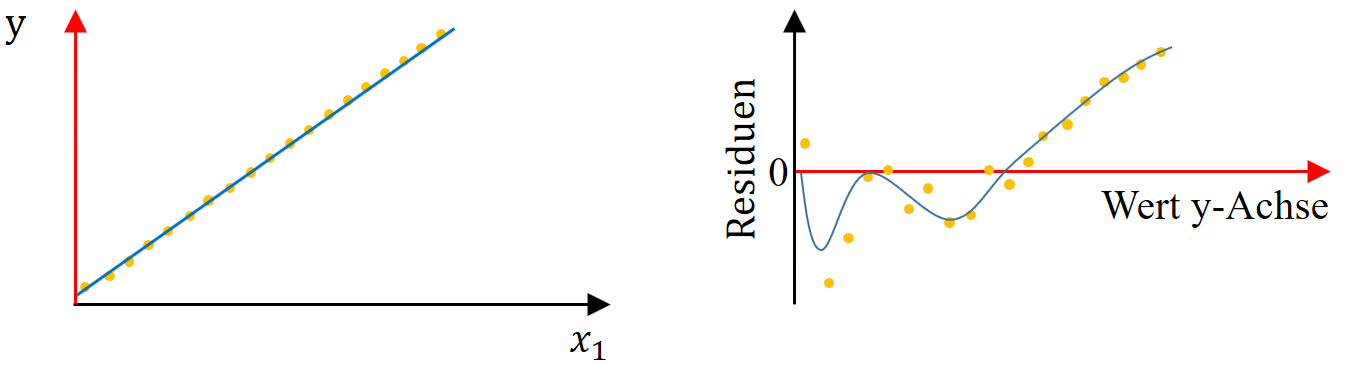
\includegraphics[width=0.6\linewidth]{figures/Residuen}
	\caption{Mit dem Tukey-Anscombe-Diagramm wird die nicht Konstant Verteilung der Residuen ersichtlich. Die gezeichnete Linie wird auch als Glätter bezeichnet}
	\label{fig:residuen}
\end{figure}
\begin{figure}
	\centering
	\subfloat[\label{subfig:residuen2} Tukey-Anscombe-Plot: \textbf{Ist Fehler symmetrisch?}  Resiuduen müssen um 0 sein und innerhalb der grauen beispiel Residuen verlaufen. Kann optimiert werden durch Transformation der erklärenden Variabel]{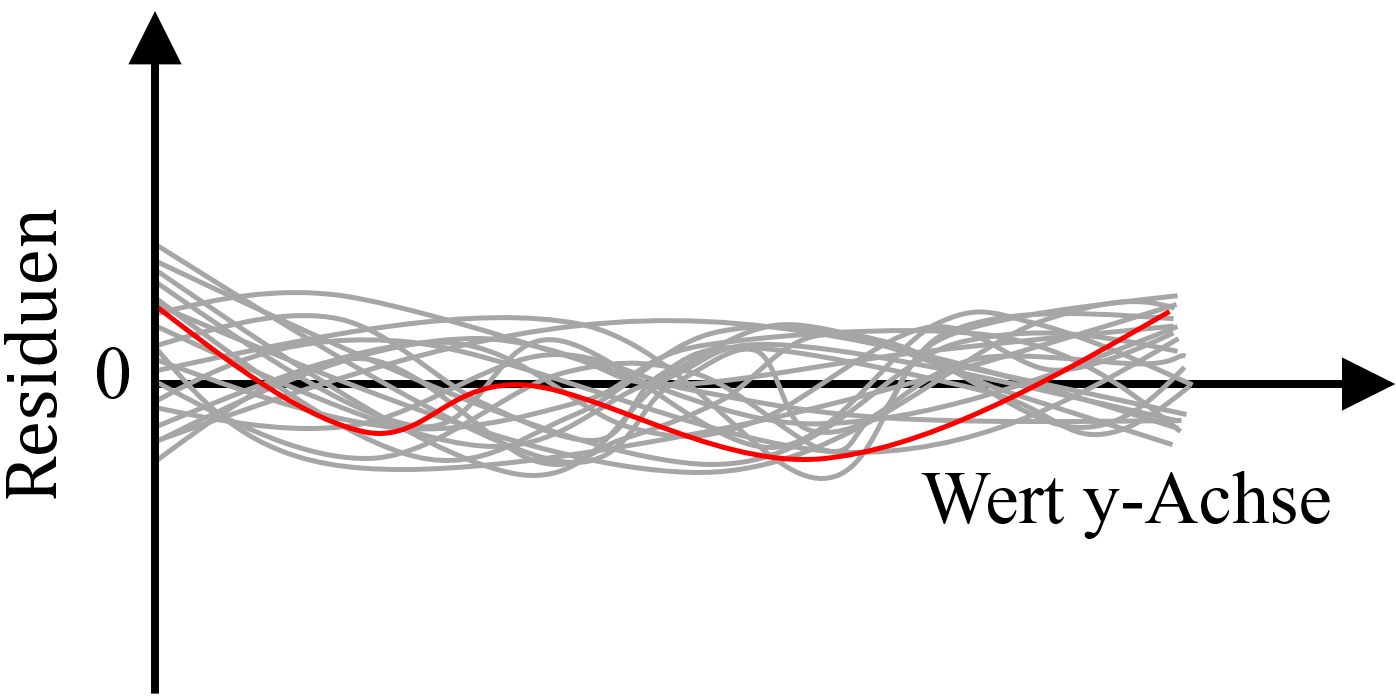
\includegraphics[width=0.25\linewidth]{figures/Residuen2}}
	\hspace{0.1\linewidth}
	\subfloat[\label{subfig:residuen3} Scale-Location-Plot\textbf{Ist Fehler konstant?} Streuung der Residuen muss konstant sein und innerhalb der grauen Beispielstreungen verlaufen, Beispiel zeigt nicht typische Verteilung der Residuen. Kann optimiert werden durch Transformation der Zielvariabel]{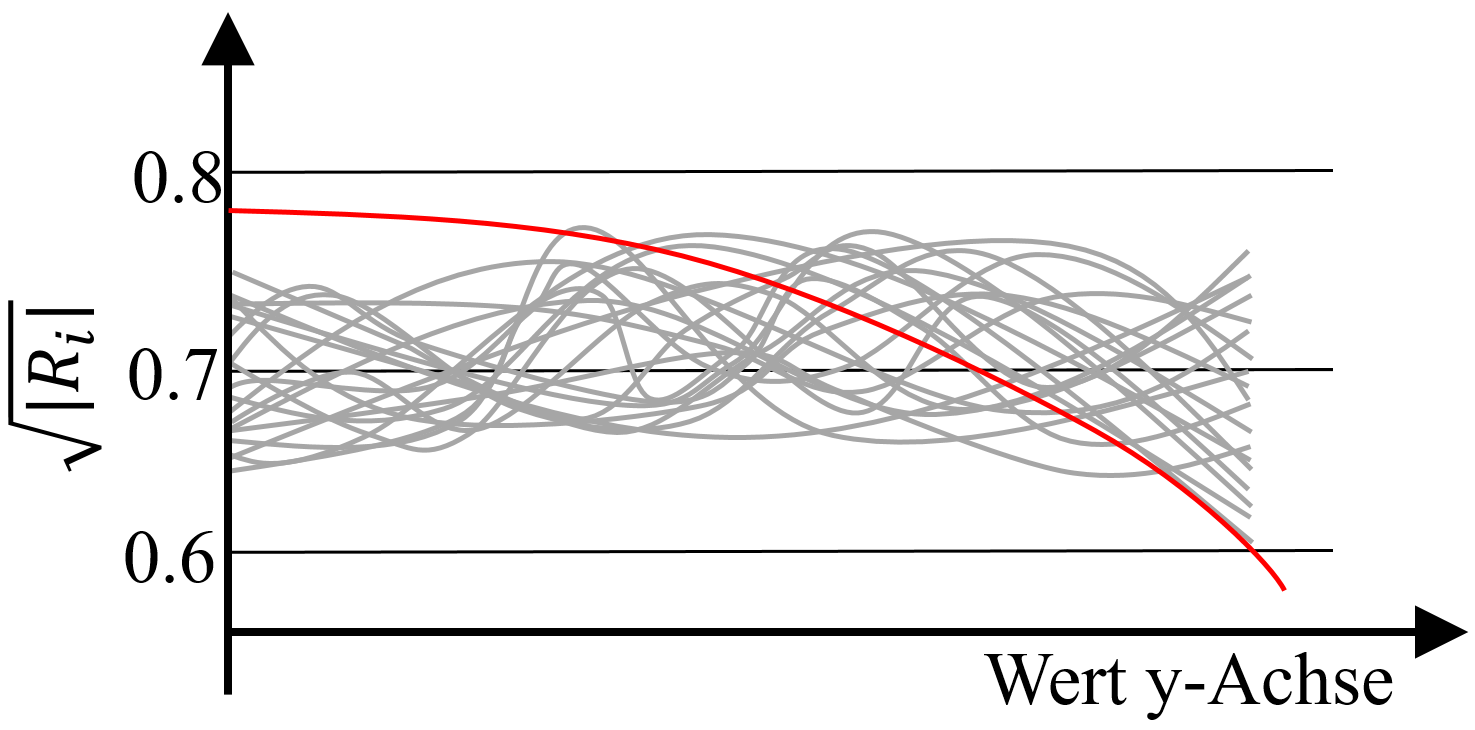
\includegraphics[width=0.25\linewidth]{figures/Residuen3}}\\
	\subfloat[\label{subfig:residuen4} Normal-Plot \textbf{Ist Fehler normalverteilt?} Quantile der empirischen Verteilung der Residuen werden mit Quantilen der Normalverteilung verglichen, \textit{Quelle:}\cite{C:theoQuantilen}]{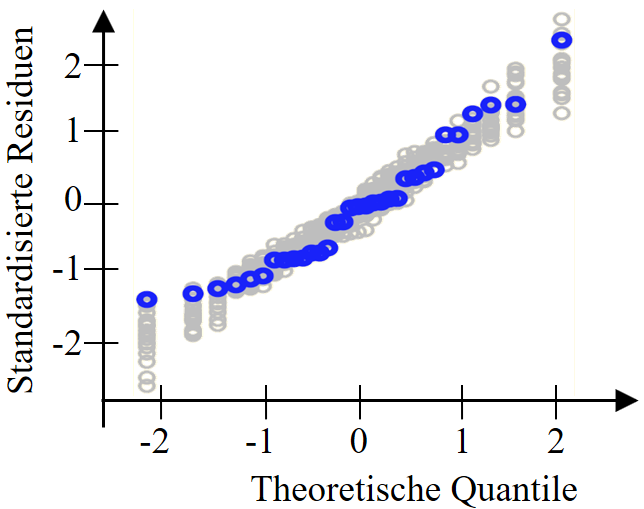
\includegraphics[width=0.2\linewidth]{figures/Residuen4}}
		\hspace{0.1\linewidth}
	\subfloat[\label{subfig:residuen5} Verlauf von langschwänzigen und kurzschäwnzigen Daten]{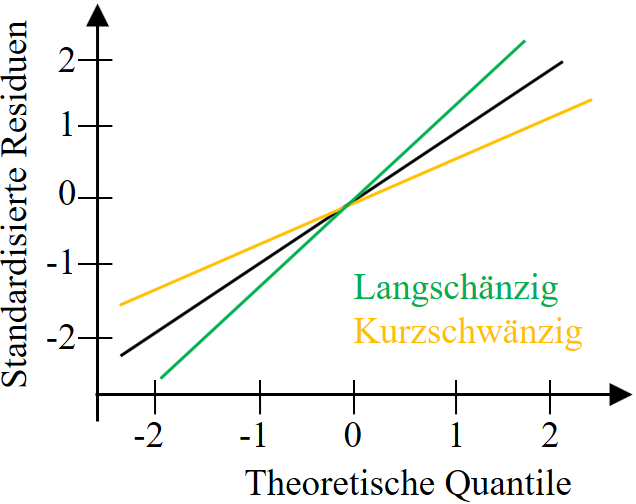
\includegraphics[width=0.2\linewidth]{figures/Residuen5}}
	\caption{Rote Kurven/Punkte müssen innerhalb der grauen Kurven/Punkte verlaufen, dann ist die Form typisch$\rightarrow$ Regression ist gut}
	\label{fig:residuen2}
\end{figure}

\subsubsection{Transofrmationen (Tukey)}
\label{subsubsec:Transformationen}
\begin{itemize}
	\item Diese Empfehlungen beruhen auf Erfahrungen
	\item Die zu verwendende Transformation hängt von dem Typ der Daten ab
	\item Sollen Defizite in der Streuungsannahme beheben
	\item Sowohl auf Ziel variablen, wie auch auf erklärende Variablen Anwenden
	\begin{itemize}
		\item Es können unterschiedliche Transformationen gleichzeitig verwendet werden, wenn z.B. die Erklärende Variabel ein Anteil ist und die Zielvariabel ein Betrag, so kann die Erklärende Variabel mit Arcus-Sinus-Wurzel-Transformation transformiert werden und die Zielvariabel mit der Logarithmus-Transformation.
	\end{itemize}
	\item Die Transformationen
	\begin{itemize}
		\item [1.] Logarithmus-Transformation für \underline{Konzentrationen und Beträge}
		\begin{itemize}
			\item Variablen dürfen kein Zeitlicher Einfluss haben, da diese sonst keine Beträge mehr sind
			\item Beträge: Vorzeichenlose Grössen
			\item Aus $Y_i = \alpha+\beta x_i+E_i$ wird damit $\log_{10}(Y_i) =\alpha+\beta\log_{10}x_i+E_i$
		\end{itemize}
		\item [2.] Die Wurzeltransformation für \underline{Zähldaten} (z.B. Anzahlen) oder wenn etwas mit jeder weiteren Probe abnimmt (z.B. in Folge von Erfahrungsgewinn)
		\item [3.] Arcus-Sinus-Wurzel-Transformation $Y_i = \arcsin(\sqrt{Y_i})$ für \underline{Anteile (Prozentzahlen)} ($\in\left[0,1\right]$)
		\item [4.] Logit-Transformation $y = \log\left(\frac{y+0.005}{1.01-y}\right)$
	\end{itemize}
\end{itemize}

\subsection{Multiple lineare Regression}
\begin{itemize}
	\item Zusammenhang einer Zielgrösse in Abhängigkeit mehrerer Ausgangsgrössen (erklärende Variablen)
	\item $Y_i = \beta_0+\beta_1 x_i^{(1)}+\beta_2 x_i^{(2)}+\ldots+\beta_3 x_m^{(m)}+E_i$
	\item $m =$ Anzahl unterschiedliche erklärende Variablen
	\item $\beta_0 =$ Achsabschnitt, Es gibt nur einen für alle Variablen geltenden Achsabschnitt 
	\item $\beta_m = $ Koeffizient der erklärenden Variabel $x^{(m)}$
	\item $\sigma^2 = $ Varianz der Abweichung $E_i$
	\item Für Beispiels eines R-Outputs siehe \ref{subsubsec:MultipleLineareRegressionR}
	\item Wenn $\text{Pr}(>\vert t \vert)$ kleiner als 0.05 (resp. Vorgegebenem Signifikanzniveau) ist, können wir nicht davon ausgehen, dass das weglassen dieser Variabel keinen Einfluss hat
	\begin{itemize}
		\item Umkehrfolge: Diese Variabel hat einen Effekt auf die Zielgrösse
	\end{itemize}
	\item Es lassen sich keine Schlüsse zum Signifikanzniveau ziehen zwischen einzelnen linearen Regressionen und multiplen linearen Regressionen
	\item Vertrauens, Prognoseintervall und Bestimmtheitsmass genau wie bei einfacher linearer Regression (siehe Gleichung \ref{eq:Vertrauensintervall}, \ref{eq:Prgronoseintervall} und \ref{eq:RSquare})
	\begin{itemize}
		\item $\eta_0 = $ Erwartungswert gemäss Berechnung
		\item $\alpha$ entspricht $\beta_0$, etc.
	\end{itemize}
	\item Polynominale multiple Regression: Wir wählen für $x^{(1)} = x$, für $x^{(2)} = x^2$ etc.  
	\begin{itemize}
		\item Somit können auch Werte von höheren Potenzen mit der normalen linearen Regression angepasst werden 
		\item Formel bleibt somit gleich $Y_i = \beta_0+\beta_1 x_i^{(1)}+\beta_2 x_i^{(2)}+\ldots+\beta_3 x_m^{(m)}+E_i$ 
	\end{itemize} 
\end{itemize}

\subsubsection{Binäre- und Faktorvariablen}
\begin{itemize}
	\item Wie der Name sagt, nimmt entweder Wert 0 oder 1 an
	\item $Y_i =\beta_0+\beta_1x^{(1)}+\ldots+\beta_ix^{(i)}+E_i$
	\begin{itemize}
		\item $x_i$ nimmt für zb. für $i<15$ den Wert 0 an, für Werte $i\geq15$ den Wert 1 an 
	\end{itemize}
	\item Wenn Variabel den Wert 1 annimmt (im Beispiel für $\beta_{15}$ ergibt sich somit: $Y_{15}=\left(\beta_0+\beta_{15}\right)+\beta_1x_{15}^{(1)}$
	\begin{itemize}
		\item Die entspricht also einer Verschiebung des Achsabschnittes um $\beta_{15}$
	\end{itemize}
	\item \textbf{Faktorvariablen} ermöglichen es den Achsabschnitt in Abhängigkeit einer Binären Variabel zu verschieben
	\begin{itemize}
		\item Beispiel: Messungen an verschiedenen Orten des gleichen Ereignisses
		\item Jeder Ort erhält eine Binäre Variabel, die genau dann 1 wird, wenn die Messung von diesem Punkt stammt
		\item Verschiebt den Achsabschnitt genau wie die binäre Variabel 
		\item [$\Rightarrow$] Mit jeder Faktorvariabel geht ein anderer Offset einher
	\end{itemize}
	\item Im Summary-Output entsprechen die $\beta$-Werte der Faktorvariablen gerade der Verschiebung des Achsabschnittes
	\item Faktorvariablen führen zu einem Block von Indikationsvariablen
	\item Siehe für Beispiel Lösung von Übungen Reg3 auf 3b
\end{itemize}

\subsubsection{F-Test (F-Statistik)}
\begin{itemize}
	\item Können alle Variablen zugleich 0 sein?
	\begin{itemize}
		\item Nullhypothese: $H_0: \beta_0 = \beta_1 =\ldots=\beta_m=0$
	\end{itemize}
	\item Wichtig ist, dass der p-Wert der F-Statistik klein ist (<0.05), dann ist 0-Hypothese widerlegt.
	\begin{itemize}
		\item Mindestens einer der Paramter (ohne $\beta_0$ ist ungleich null (und beeinflusst somit die Zielvariabel)
	\end{itemize}
	\begin{itemize}
		\item F-Statistik (...) on x and y DF
		\item x: Anzahl Parameter (ohne $\beta_0$) $\rightarrow$ Anzahl unterschieldiche Steigungen
		\item y: Anzahl Datenpunkte (Anzahl Zeilen der Daten) minus Anzahl der zu bestimmenden Parameter (mit $\beta_0$)
	\end{itemize}
\end{itemize}

\subsubsection{Wechselwirkung}
\begin{itemize}
	\item Wechselwirkung zwischen zwei grössen kann untersucht werden mit:
	\begin{itemize}
		\item \textit{myVar.lm $<-$ lm(A$\sim$X$\ast$Y,data=myDat}
		\item [] \textit{summary(myVar.lm)}
	\end{itemize}
	\item Die Zeile \textit{X:Y (...)} im Output gibt an
	\begin{itemize}
		\item Spalte Estimate: A $\rightarrow$ Steigungsunterschied von X zu Y $\rightarrow$ Wenn $A>0$ hat X eine um A grössere Steigung als Y
		\item Signifikanzlevel: zeigt an bei welchem Signifikanzlevel diese Wechselwirkung signifikant wird
	\end{itemize}
\end{itemize}


\subsection{Sensitivität und Robustheit}

\subsubsection{Senitivität}
\textbf{Cooksdistance}
\begin{itemize}
	\item Wie starkt beeinfflusst eine Beobachtung (insbesondere ein Ausreisser) die Analyse?
	\item Die Distanz von Cook $d_i$ prüft wie fest ein Wert die Schätzung ($\hat{y}_i$) beeinflusst
	\begin{itemize}
		\item Reminder: $\hat{y}_i$ ist der Wert der mit der linearen Regression berechnet wird
		\item Also wird der Einfluss auf die Regressionsgerade (oder Ebene, oder etc.) betrachet
		\item Wert ist normiert mit $p\cdot\hat{\sigma}^2$
	\end{itemize}
	\item Zu einflussreich sind Werte mit einer Cook's Distanz von grösser als 1
\end{itemize}
\textbf{Hebelarm (leverage)}
\begin{itemize}
	\item $h_i$ ist Einfluss der erklärenden Variabel, Wertebereich $0\leq h_i \leq 1$
	\item Die Senitivitätsanalyse mit $h_i$ ist nur bei einzelnen Ausreisser hilfreich, nicht bei Gruppen von Ausreissern
	\item Wenn eine Beobachtung $Y_i$ um $\Delta y_i$ verändert wird, dann ist $h_i\cdot\Delta y_i$ die Veränderung von dem mit der  Regression berechneten Wertes $\hat{y_i}$
	\item Generell gilt, wenn der Hebelarm $h_i<0.2$ ist, ist die Beobachtung unbedenklich
\end{itemize}
\textbf{Punkte identifizieren mit zu grossem Einfluss}
\begin{itemize}
	\item Werden der Hebelarm und die Cooksche-Distanz in einem kombiniert, können damit zu Einflussreiche Punkte identifiziert werden
	\item In Abbildung \ref{fig:sensitivitaet} ist ein solches Diagramm gezeigt, alle standardisierten Fehler $\hat{\sigma_i}$ werden in dieses Eingetragen
	\begin{itemize}
		\item Solange diese Innerhalb der erlaubten Cookschen Distanz (meistens 1) sind ist es kein Problem
		\item Punkte Ausserhalb der Cookschen Distanz haben in y-Richtung einen zu grossen Einfluss
		\item Beobachtungen mit einem Hebel Oberhalb von $h_i>0.2$ haben einen grossen Einfluss auf die Regressionsgerade
		\item Nur Hebelpunkte ($>0.2$) ausserhalb der Cookschen Distanz sind einflussreich
		\begin{itemize}
			\item Solange diese Jedoch innerhlab der Cookschen Distanz liegen sind dies keine Ausreisser und beeinflussen die Regression nicht negativ
		\end{itemize}
	\end{itemize}
\end{itemize}

\begin{figure}[h!]
	\centering
	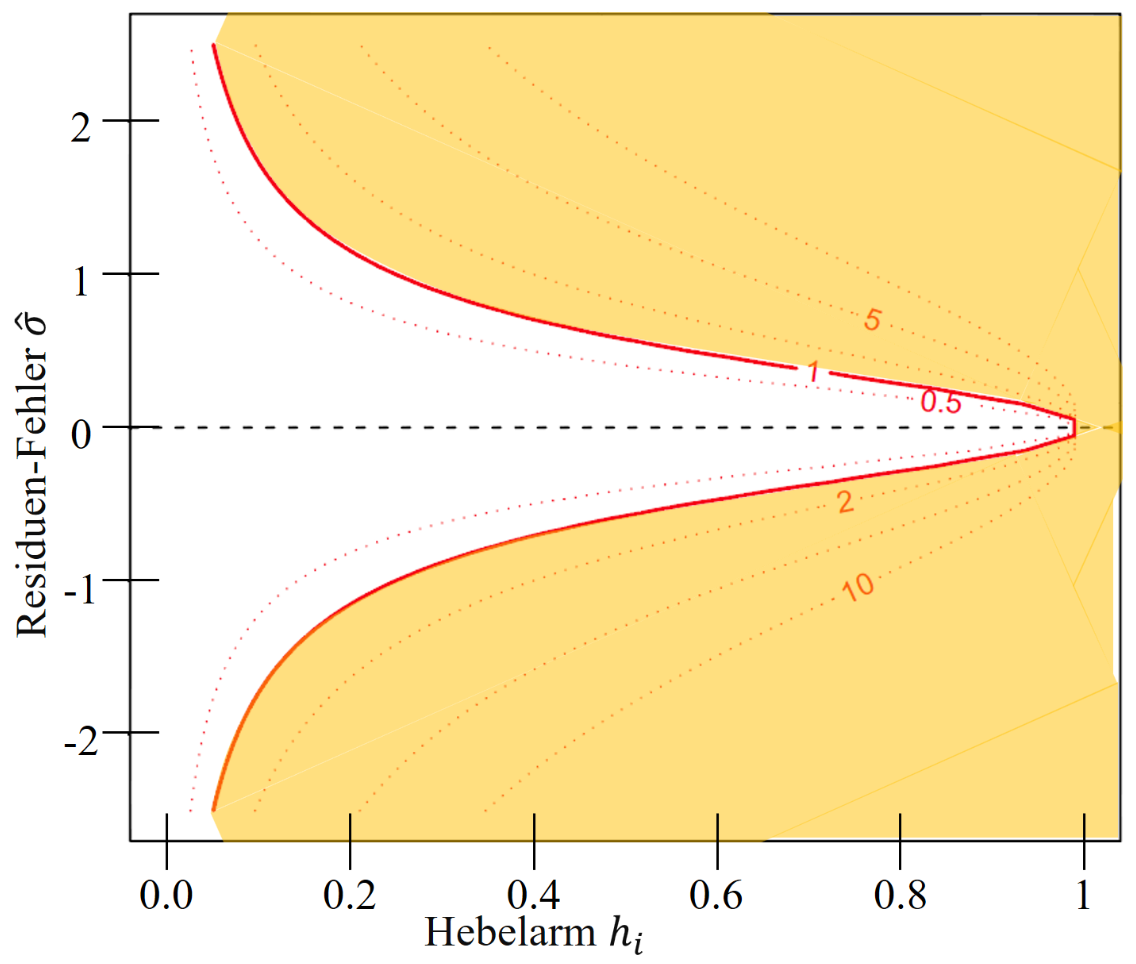
\includegraphics[width=0.3\linewidth]{figures/Sensitivitaet}
	\caption{Sensitivitätsanalyse: Diagramm um Ursache des zu grossen Einflusses zu identifizieren \textit{Quelle: }\cite{C:Cook}}
	\label{fig:sensitivitaet}
\end{figure}

\subsubsection{Gewichtete Lineare Regression}
\begin{itemize}
	\item NoS = Number of Samples
	\item Bei mehreren Beobachtungen denjenigen mit der kleineren Streuung in der Regressionsrechnung das grössere Gewicht geben
	\item \textit{lm(YAches$\sim$XAchse,data = myData, \underline{weights=NoS}}
	\begin{itemize}
		\item Je mehr Samples von einer Probe vorliegen desto grösser wird diese gewichtet
	\end{itemize}
	\item Wenn dies so eingesetzt wird, sollte der zur F-Statistik gehörende p-Wert besser sein, als ohne die Gewichtung.
\end{itemize}

\subsubsection{Robustheit}
\begin{itemize}
	\item Definition von Robustheit
	\begin{itemize}
		\item Ein Ausreisser $P_1$ mit einer kleiner Abweichung von der Normalverteilung hat nur eine kleine Auswirkung auf das Modell
		\item Ein Schätzverfahren, dass die Parameter so schätzt als wäre keine Abweichung vorhanden, wird robust oder resistent genannt
	\end{itemize}
	\item Ein Alter und nicht formeller Ansatz für Robustheit ist:
	\begin{itemize}
		\item Prüfen der Daten auf Ausreisser, diese Ausreisser löschen und Anschliessend modell mit dem verkleinerten Datensatz erstellen
		\item Kein sauberer Ansatz, da es schwer bis unmöglich sein kann Ausreisser als solche von regulären Daten auseinander zu halten. Weiter ist es schwer diesen Prozess zu formalisieren. Weiter Punkte auf Folie 16 von Reg4
	\end{itemize}
\end{itemize}

\subsubsection{Robuste Schätzer (MM-Schätzer)}
\begin{itemize}
	\item Robust Schätzer sollen die Koeffizienten so errechnen, dass Anforderungen an Robustheit und Sensitivität erfüllt werden
	\item \textit{rlm(YAchse$\sim$XAchse, data=myData)} ist ein Robuster Schätzer, aber
	\begin{itemize}
		\item Dieser Berücksichtigt keine Hebelpunkte, sondern korrigiert nur zu grosse Residuen
	\end{itemize}
	\item \textit{lmrob(YAchse$\sim$XAchse, data=myData)} ist ein Robuster Schätzer. 
	\begin{itemize}
		\item Kann sowhol mit grossen Residuen als auch mit Hebelpunkten umgehen
		\item Für Code interpreatation siehe \ref{subsubsec:RobSchaetzer}
	\end{itemize}
	\item Schätzungen mit den kleinsten Quadraten sind ebenfalls ungeeignet, wenn kontaminierte Beobachtungen vorliegen
	\item \textbf{Achtung:} Die Schätzung mit den kleinsten Quadraten kann gut aussehen. Obwohl die Daten ungeeignet sind. In diesem Fall, würde das Auffallen im Robusten Schätzer. Werden die schlechten Daten für die kleinst-Quadrate Methode weggelassen, ergibt diese dann das Gleiche wie der Robuste Schätzer. Andernfalls weisen die Koeffizienten $\beta_m$ massive Abweichungen auf. 
\end{itemize}

\subsection{Variablenselektion}
\begin{itemize}
	\item Nur im Idealfall ist bekannt, das $Y$ von den gegebenen Variablen linear abhängig ist
	\item Im anderen Fall muss der Zusammenhang zwischen $Y$ und den Variablen zuerst hergestellt werden
\end{itemize}

\subsubsection{Adjusted $R^2$, Modellwahlkriterien}
\begin{itemize}
	\item Variabelselektion beruht auf Kriterien, die Güte durch eine statistische Messzahl beschreiben. 
	\begin{itemize}
		\item Diese sollte einerseits Modellgenauigkeit und die Modellkomplexität beschreiben
		\item Komplexität: Wie viele Parameter müssen ermittelt werden
		\item Das sind zwei gegensätzliche Anforderungen
	\end{itemize}
	\item $R^2$ ist eine untaugliche Zahl um als Modellwahlkriterium, da die Modellkomplexität nicht berücksichtigt wird
	\item Das korrigierte Bestimmtheitsmass \textit{Adjusted }$R^2$ trägt dem Rechnung. Berechnet gemäss Formel \ref{eq:AdjR2}
	\begin{itemize}
		\item Dabei ist $n$ die Anzahl der Beobachtungen (Anzahl der Datenpunkte)
		\item und $p$ ist die Anzahl unbekannte Paramter ohne $\sigma$ also Anzahl der $\beta$ (inkl. $\beta_0$)
		\item Achtung: Wenn berechnet werden muss, in Output ist bereits $R^2$ gegeben, nicht mehr quadrieren für Term $1-R^2$
	\end{itemize}
\end{itemize}

\subsubsection{AIC-Kriterium}
\begin{itemize}
	\item bestes verallgemeinertes Kriterium
	\item Formel \ref{eq:AIC} für Berechnung, dabei gilt
	\begin{itemize}
		\item $p^\diamond$  Anzahl geschätzte Parameter (inkl. $\sigma$)
		\item $SS_E$ Summe der quadrierten Residuen
		\item $n$ Anzahl der Beobachtungen
	\end{itemize}
	\item R! versucht wählt jeweils die Option die den AIC-Wert so weit wie möglich ins minus bringt
	\begin{itemize}
		\item Sobald im Output der Wert \glq none \grq den kleinsten Wert hat, wird suche abgebrochen
		\item Beispiel für Schrittweise Selektion in Kapitel \ref{subsubsec:AIC} (Abbildung \ref{fig:aic})
		\item Der default-Wert für die Richtung von step ist \glqq backward \grqq
	\end{itemize}
\end{itemize}
\begin{align}
	\label{eq:AdjR2}
	R_{adj}^2 &=1-\frac{n-1}{n-p}\left(1-R^2\right)\\
	\label{eq:AIC}
	\text{AIC}&= -2\text{(maximierte Log-Wahrscheinlichkeit)} +2\text{Anzahl geschätzte Parameter}
			  &=n \log\left(\frac{1}{n}SS_E\right)+2p^\diamond+Konstante
\end{align}



\subsubsection{Methoden zur Variablenselektion }
\begin{itemize}
	\item Modellwahl: Wahl mit welchen Variablen unser Modell gemacht wird
	\item Achtung: Alle Modellwahlkriterien garantieren nicht das global optimale Modell zu finden
	\begin{itemize}
		\item Der einzige Weg dieses zu finden, ist alle möglichen Kombinationen durchzuprobieren.
		\item All-Subset Selection
		\item Wenn das $m$ (Anzahl der erklärenden Variablen) gross ist, ist Rechenaufwand dafür riesig
	\end{itemize}
	\item Es sollten immer mehrere Modell in Betracht gezogen werden, welche von den Kriterien als gut bewertet sind
	\begin{itemize}
		\item Meist ist das an den Kenngrössen (z.B. $R_{adj}^2$) gemessene, zweitbeste Modell nicht viel schlechter als das\glqq beste \grqq
		\item Es heisst nicht, das das Modell mit dem grössten $R_{adj}^2$ das \glqq wahre \grqq Modell ist.
	\end{itemize}
	\item \textbf{Vorwärtselektion}
	\begin{itemize}
		\item Anfangsschritt: $Y_i=\beta_0+E_i \Leftrightarrow$ \textit{lm(Y$\sim$ 1,...)}
		\item Nehme jeweils diejenige Variabel in das Modell, die zur grössten Verbesserung (Vergrösserung) von $R_{adj}^2$ führt
		\item Stoppregel: Sobald keine Verbesserung mehr erfolgt durch hinzunehmen der nächsten Variabel (alle durchprobieren!)
	\end{itemize}
	\item \textbf{Rückwärtsselektion}
	\begin{itemize}
		\item Beginne mit einer Linearenregression mit allen Variablen \textit{lm(Y$\sim$.,...)}
		\item Lasse jeweils diejenige Variabel vom Modell weg, sodass die zur grösste Verbesserung (Vergrösserung) von $R_{adj}^2$ erreicht wird
		\item Stoppregel: Sobald keine Verbesserung mehr erfolgt durch weglassen der nächsten Variabel (alle durchprobieren!)
	\end{itemize}
	\item \textbf{Schrittweise Selektion}
	\begin{itemize}
		\item Kombination aus Vorwärtsselektion und Rückwärtsselektion.
		\item Bei jedem Schritt probieren, ob das Hinzunehmen oder das Weglassen einer Variablen zum bessern Ergebnis führt
		\item Immer das mit dem besten Ergebnis umsetzen
		\item Stoppregel: Keine Verbesserung mehr möglich
	\end{itemize}
\end{itemize}

\subsubsection{Kollinearität}
\begin{itemize}
	\item Definition: Eine Erklärendevariabel lässt sich als Summe anderer erklärender Variablen darstellen
	\item Hohe Kollinearität zwischen erklärenden Variablen sind von der Theorie her zugelassen, geben jedoch beim Interpretieren und statistischen Modellieren des Modells Probleme
	\begin{itemize}
		\item Bei obigen Verfahren (Vorwärtsselektion, etc.) kann es vom Zufall abhängen, welche Variabel als erstes gewählt wird
	\end{itemize}
	\item \textbf{Variance inflation factor (VIF)} ist das Mass das Aussagen über die Kollinearität zu den anderen Variablen gibt
	\begin{itemize}
		\item Wenn dieses Mass hoch ist, (grösser als 5 bis 10) ist ein Problem mit der Kollinearität vorhanden
		\item Für jede Variabel $x^{(j)}$ gegenüber jeder anderen Variabel das $R_j^2$ dieser Variabel berechnen, daraus das VIF gemäss Formel \ref{eq:VIF} berechnen
	\end{itemize}
	\item Für R!-Output siehe \ref{subsubsec:VIF}
	\begin{itemize}
		\item Korrelierende Werte haben hohen VIF-Wert
		\item Zudem ist zu  erkennen, dass diese gegeneinander aufgetragen in den Diagrammen eine Gerade bilden!
	\end{itemize}
	\item Gegenmassnahmen Kolinearität:
	\begin{itemize}
		\item Bereits bei Beobachtungen versuchen diese zu vermeiden (Wahl der beobachteten Grössen)
		\item Wenn dies nicht möglich ist: Stark korelierende Variablen ersetzen durch ihre Summe und ihre Differenz (falls dies sinnvoll ist)
		\item ggf. Variabel mit dem höchsten VIF aus dem Modell entfernen
	\end{itemize}
\end{itemize}

\begin{align}
	\label{eq:VIF}
	\text{VIF}_j &= \frac{1}{1-R_j^2}
\end{align}

\subsubsection{Vorgehen (vereinfacht)}
\begin{itemize}
	\item [1.] Problem verstehen, gibt es Modellansätze?
	\item [2.] Daten Aufbereiten
	\begin{itemize}
		\item Umgang mit fehlenden Daten
		\item Bedeutung von 0 in verschiedenen Variablen vereinheitlichen
		\item Daten mit Tukey behandeln falls nichts dagegen spricht
	\end{itemize}
	\item [3.] Erste Anpassung am besten mit Robuster MM-Methode
	\item [4.] Residuen Analyse, tragen Daten dazu bei das Problem zu lösen, allenfalls zurück zu 1 oder 2
	\item [5.] Variabelselektion
	\item [6.] Modelleignung klären
	\begin{itemize}
		\item Residuen mit gewählten Variablen
		\item Modell vergleichen mit Fachwissen, plausibilität?
		\item Validierung des Modells wenn möglich (mit noch nicht verwendeten oder neuen Daten)
	\end{itemize}
\end{itemize}
\clearpage

\section{Designe of Experiment}
\subsection{Wichtige Wörter}
\begin{itemize}
	\item \textbf{Experiment:} Subjekte oder Objekte einer bewusst geschaffene Situation werden beobachtet
	\begin{itemize}
		\item Kausale Zusammenhänge lassen sich besser durch Experimente zeigen (Einflussgrössen frei einstellbar)
	\end{itemize}
	\item \textbf{Erhebung:} Subjekte oder Objekte werden im Rahmen einer existierenden Situation beobachtet
	\begin{itemize}
		\item Meist zu viele Variablen, Interpretation wird schwierig
	\end{itemize}
	\item \textbf{Statistischer Versuchsplanung - DoE:} Planung, sodass Daten mit statistischen Methoden zielführend ausgewertet werden können
	\begin{itemize}
		\item Möglichst wenige Messungen, für möglichst präzise Schätzungen oder möglichst mächtige Tests
	\end{itemize}
	\item Variablen-Screening um wichtige Grössen zu identifizieren (Screening-Experiment), besonders bei vielen Variablen
	\item \textbf{Primäre Variablen od. Prüffaktoren:} Hauptfrage an das Experiment hängt direkt mit diesen Variablen zusammen
	\begin{itemize}
		\item Bei einer Primären Variabel: Zwei möglichst weit auseinanderliegende Einstellungen wählen, und dazwischen gleichmässig verteilte Werte prüfen
		\item Bei mehreren Primären Variablen: Variablen sollten möglichst orthogonal sein zueinander (Keine Korelation zwischen einzelnen Variablen)
	\end{itemize}
	\item \textbf{Sekundär Variablen od. Störfaktoren:} Feststellbarer Einfluss auf das Ergebnis des Experiments, müssen nicht zwingend kontrollierbar sein
	\item \textbf{Blockbildung:} mit \glqq künstlichen \grqq Variablen, z.B. für Batches, Produktions-Lose, etc. 
	\item \textbf{Replikate:} Führen zu höheren Genauigkeit, keine Scheinwiederholungen (Messungen gleich nacheinander $\rightarrow$ Randomisieren)
	\item \textbf{Versuchsplan:} Liste aus Versuchsbedingungen, z.B. Welcher Faktor auf welchen Stufen variiert wird
	\begin{itemize}
		\item Vollständig randomisierter Versuchsplan: Bei einem Faktor mit mehreren Stufen mehrere Messungen pro Stufe (aber immer gleich viele). Abarbeitung in Zufälliger Reihenfolge
		\item Block Design: Neben dem Primären Faktor hat es auch ein sekundärer (Stör-) Faktor mit Einfluss auf die Zielvariabel.  Kommt jede \textbf{Stufe} des ersten Faktors in jedem Block mindestens einmal zur Anwendung: Versuchsplan mit vollständigen Blöcken
		\item \textbf{Faktorielle Versuchspläne:} Versuchsplan mit Stufenkombinationen: bei $k$ Primären Faktoren mit je $L$ Stufen. Werden alle Kombinationen getestet ($L^k$ Messungen) ist das der vollständig faktorielle Versuchsplan
		\begin{itemize}
			\item Wenn keine Wechselwirkungen zwischen den Variablen, können unvollständige Versuchpläne eingesetzt werden. Sind diese immernoch ausgewogen (balanciert) sind das fraktionelle Versuchspläne
			\item Haben die Faktoren im vollständig faktoriellen Versuchsplan nur zwei Stufen, dann ist das ein vollständiger $2^k$-faktorieller Versuchsplan (für jeden Faktor werden zwei Messungen gemacht)
		\end{itemize}
	\end{itemize}
\end{itemize}


\subsection{Faktorielle Designs}
\begin{itemize}
	\item Oftmals auch als Varanz-Analyse bezeichnet
	\item Eine Zielgrösse interessiert uns, die nicht direkt messbar ist, jedoch durch Faktoren beeinflusst wird
	\begin{itemize}
		\item z.B. verschiedene Level, Methoden, etc. Alles sind diskrete und nicht kontinuierliche Werte
		\item Es handelt sich also um Faktorvariablen (so z.B. Level 5\%, Level 10\%, Level 15\% oder Methode 1, Methode 2, etc.)
	\end{itemize}
	\item Kann gut in Notch-Box-Plot dargestellt werden (siehe Abbildung \ref{fig:notchedboxplot}). Ein dieser Plots pro gemessenem Level (z.B. Konzentration 5\%, Konzentration 10\%, etc.) In Y-Achse die zu bestimmende Variabel
\end{itemize}
\begin{figure}[h]
	\centering
	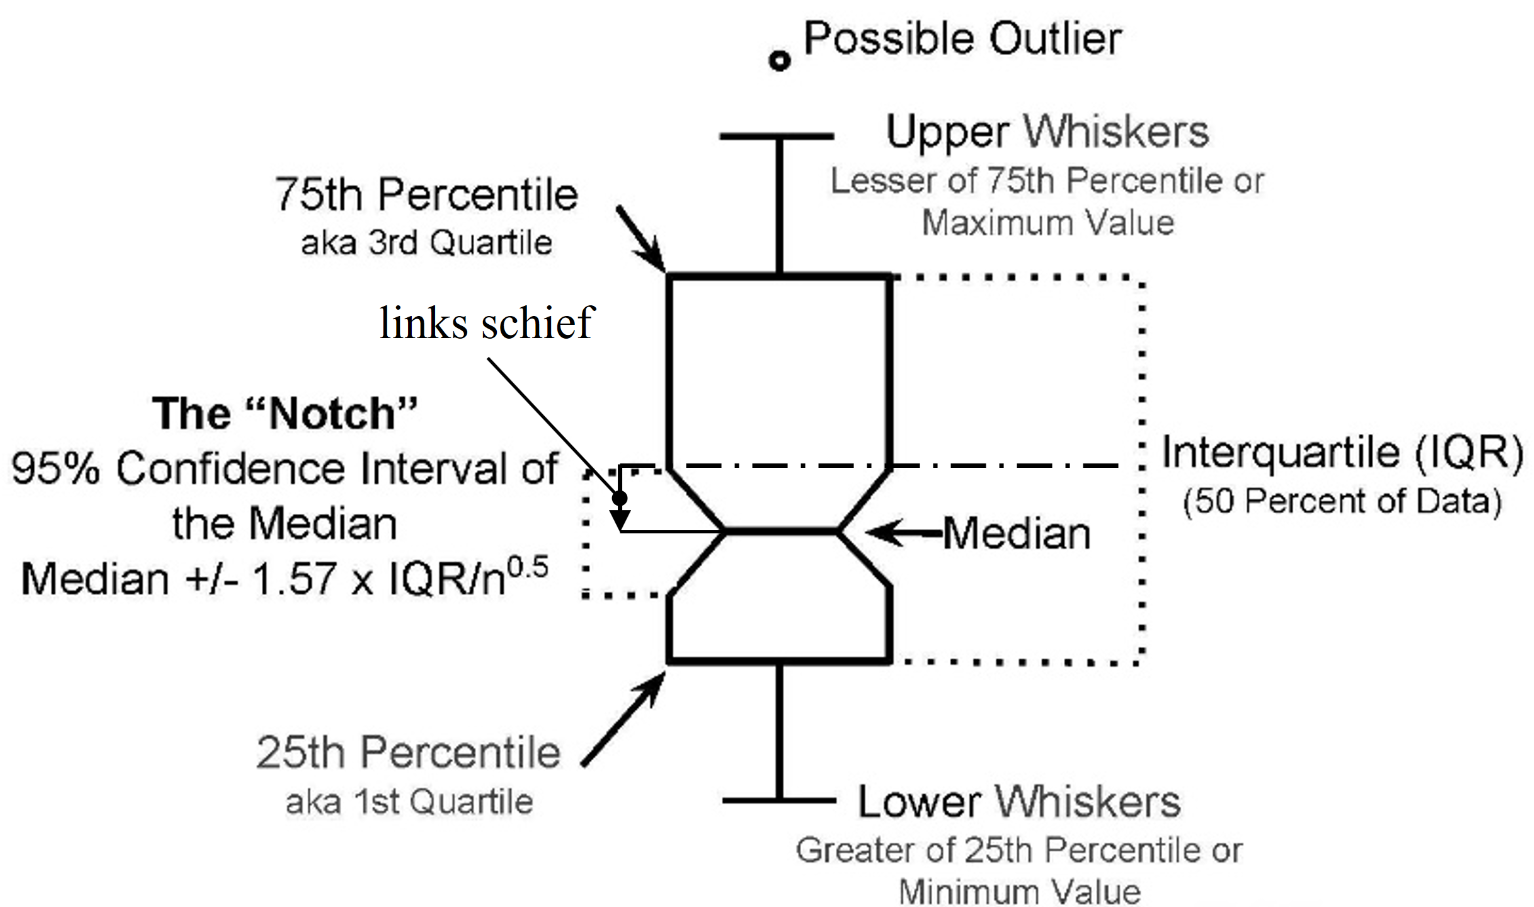
\includegraphics[width=0.5\linewidth]{figures/NotchedBoxPlot}
	\caption{Notch-Boxplot mit Kenngrössen \textit{Quelle:} \cite{C:NotchBoxPlot}}
	\label{fig:notchedboxplot}
\end{figure}

\subsubsection{Anova-Test}
\label{subsubsec:AnovaTest}
\begin{itemize}
	\item Teststatistik die extreme Werte annimmt, wenn sich die Gruppen in er Lage unterscheiden
	\begin{itemize}
		\item Das heisst, wenn der Mittelwert der einzelnen Gruppen auf unterschiedlicher Höhe liegt
		\item In diesem Fall kann die 0-Hypothese verworfen werden (da sich die Ergebnisse einzelner Gruppen signifikant unterscheiden). Es kann somit davon ausgegangen werden, dass die einstellungen der Gruppen das Resultat beeinflussen. 
		\item In Abbildung \ref{fig:Anova} ist gezeigt, wie ein solcher Test aufgebaut ist. Die Ausgabe ist der Quotient zwischen der Streuung zwischen den Gruppen und der Streuung innerhalb der einzelnen Gruppen
		\item Dieser Koeffizient wird als $T$ bezeichnet in der Abbildung ist dieser rot hinterlegt. 
		\item Wenn im R-Output das Signifikanzlevel (Pr($>$F)) klein ist, kann die $H_0$ des F-Tests abgelehnt werden. Mindestens eine der gemessenen Gruppen hat Einfluss. 
	\end{itemize}
	\item Siehe \ref{subsec:RBefehler} für die Anwendung für Wechselwirkungen
\end{itemize}

\begin{figure}[!h]
	\centering
	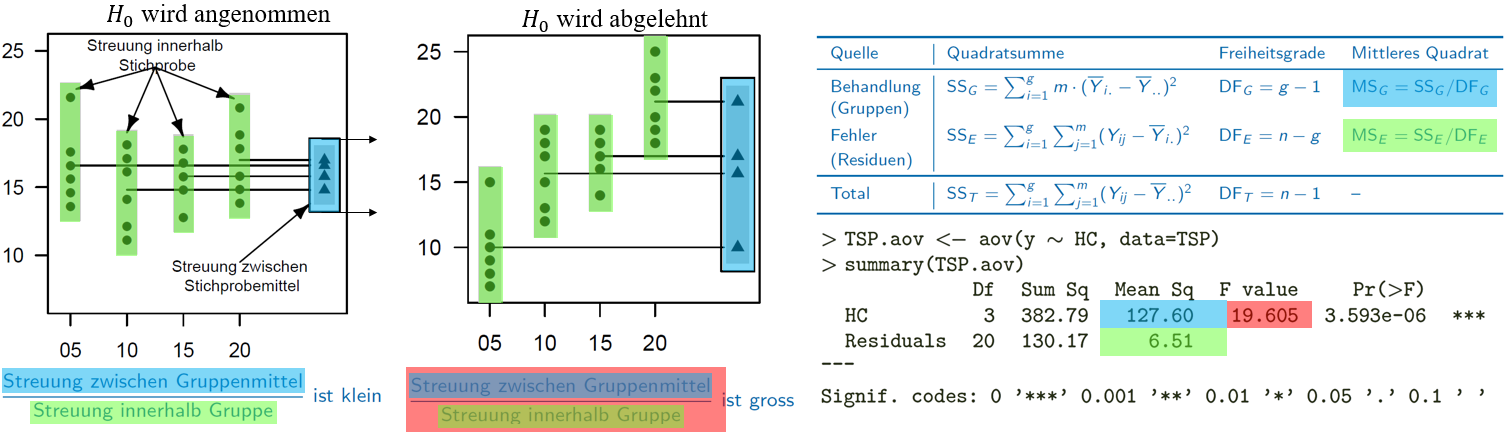
\includegraphics[width=1\linewidth]{./figures/Anova.png}
	\caption{Schema des Anova-Tests. Dieser gibt Auskunft ob $H_0$ über Gruppen abgelehnt oder angenommen wird. \textit{Quelle:}\cite{C:Anova}}
	\label{fig:Anova}
\end{figure}

\subsubsection{Block-Versuchsplan}
\begin{itemize}
	\item Faktor A ist ein primärer Faktor (Behandlungsfaktor)
	\item Faktor B teilt Versuch in Blöcke ein, sekundärer Faktor
	\begin{itemize}
		\item Blöcke sollten möglichst homogen sein, dass Unterschiede innerhalb des Blockes möglichst auf unterschiedliche Behandlungen zurückzuführen ist. 
	\end{itemize}
	\item Man spricht von einem Block-Design
	\item Verlaufen die Linien im Interaction Plot parallel, so kann von Addivität ausgegangen werden
	\begin{itemize}
		\item Y-Achse ist Wechselwirkung zwei verschiedener grössen
		\item X-Achse ist ein Faktor (vorteilhaft ein Primärer Faktor)
	\end{itemize}
\end{itemize}

\textbf{Zwischenstand: bis und mit DoE2}

\newpage
\section{R!-Relevante Dinge}
\subsection{Befehle}
\label{subsec:RBefehler}
\begin{tabularx}{\linewidth}{p{0.15\linewidth} X X}
	\textbf{Funktion}	&	\textbf{Befehl} 							&\textbf{Kommentar}\\\hline
	Plot erstellen		& \textit{plot(YAchse$\sim$XAchse,data=VarName)}&Namen der Y- und X-Achse müssen Spaltennamen in der Variabel
																		 sein\\\hline
	Lineare Regression	&\textit{lm(YAchse$\sim$XAchse,data=VarName)}	&Liefert Koeffizienten für lin. Regression der Y-Achse auf
																		X-Achse. \newline
																		Intercept = $\alpha$\newline
																		VarNameX  = $\beta$ der betroffenen Variabel\newline
																		Ouput von summary eines linearen eines Parameter \ref{subsubsec:summary} \\
						&\textit{lm(YAchse$\sim$X1Achse+X2Achse,data=VarName)}	
																		&Multiple lineare Regression, möglich mit beliebige vielen \textit{XnAchsen}, Summary-Output von einem Modell für multiple lineare Regression: Kapitel \ref{subsubsec:MultipleLineareRegressionR}\\\hline
	Zusammenfassung		&\textit{summary(varname)}						&Liefert die Zusammenfassung eines Elements, varname kann 
																		z.B. in von lm-Erhaltene Var sein, siehe \ref{subsubsec:summary}\\\hline
	Lin. Koeffizienten eintragen&\textit{abline(varName)}				&Zeichnet die Lin. Regression in eine Grafik, varName vom
																		 Typ \textit{lm}\\\hline
	Eine Spalte ansprechen&\textit{varName\$SpaltenName}				&Spricht eine Spalte der Variabel an, kann auch gebraucht
																		 werden um eine Spalte hinzuzufügen
																		 z.b. \textit{A\$x$<-$1/A\$B} spalte x $=\frac{1}{B}$\\\hline 
	Konfidenzintervall	&\textit{confint(lm-objekt, $\left[\text{\textit{parm=2}}\right]$,level=confLvl)}
																		&Konfidenzintervall, damit Konfidenzlevel\% der Werte 
																		innerhalb dieses
																		Bereiches ist. Bei mehreren Parameter kann optional der gewünschte Parameter angegeben werden, wenn nichts angegeben gibt Wert für alle Parameter. Somit liegt für z.B. 99\% $\rightarrow$ und parameter 2 (Steigung): Steigung muss zwischen den zwei Ausgegebenen Werten für 0.5\% und 99.5\% liegen, um ein Konfidenzintervall von 99\% zu erreichen.\\\hline
	Vertrauens- und Prognoseintervall &sieh Kapitel \ref{subsubsec:VertrauensUndPrognoseintervall}&Entsprechen Kapitel
																		 \ref{subsubsec:VertrauensUndPrognoseBereich}\\\hline
	Eine Eintrage weglassen&\textit{myData$\left[\right.$-19,$\left.\right]$}& Lässt den Datenpunkt 19 Weg\\
						&\textit{...(YAchse$\sim$XAchsee,data=myVar, subset=-19)}&Lässt überall den Eintrag 19 Weg\\\hline
	Anova-Test			&aov(YAchse$\sim$X1Achse+X2Achse,data=myData)	&F-Statistik für die zwei Beobachtungen X1 und X2\\
						&aov(YAchse$\sim$X1Achse$\ast$X2Achse,date=myData)&F-Statistik für die zwei Beobachtungen X1 und X2, inkl. 
																		der. Relevanz deren Wechselwirkung. Wechselwirkung in Output dargestellt als X1:X2. Wenn p-Wert $>0.05$ kann $H_0$ \underline{nicht} verworfen werden, d.h. Es kann sein, dass diese Wechselwirkung \underline{keinen} Einfluss hat.\\\hline
	Daten eingeben		&\textit{data.frame(...)}						&Siehe Kapitel \ref{subsubsec:Dataframe}\\\hline
\end{tabularx}

\clearpage
\subsection{Deutung des R!-Outputs}
\subsubsection{Summary}
Achtung: Ggf. ist das mit dem T-Wert nicht korrekt! Falls nötig und Zeit noch prüfen!
\label{subsubsec:summary}
\begin{figure}[h!]
	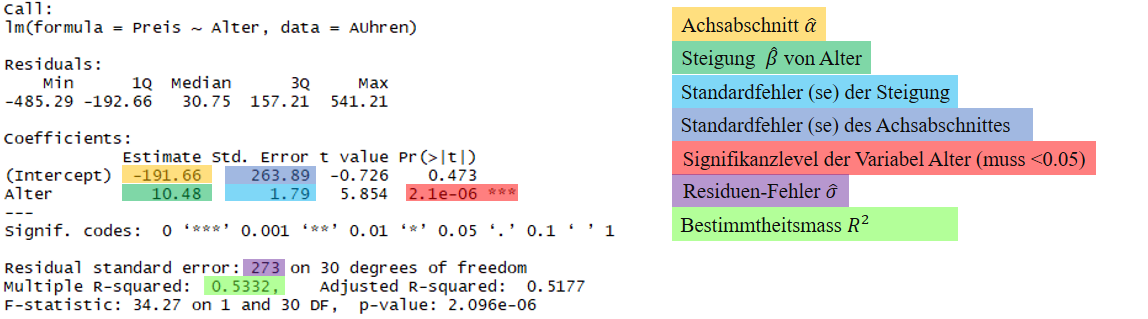
\includegraphics[width=0.9\linewidth]{figures/RSummary}
\end{figure}

\subsubsection{Vertrauens- und Prognoseintervall}
\label{subsubsec:VertrauensUndPrognoseintervall}
\begin{figure}[!h]
	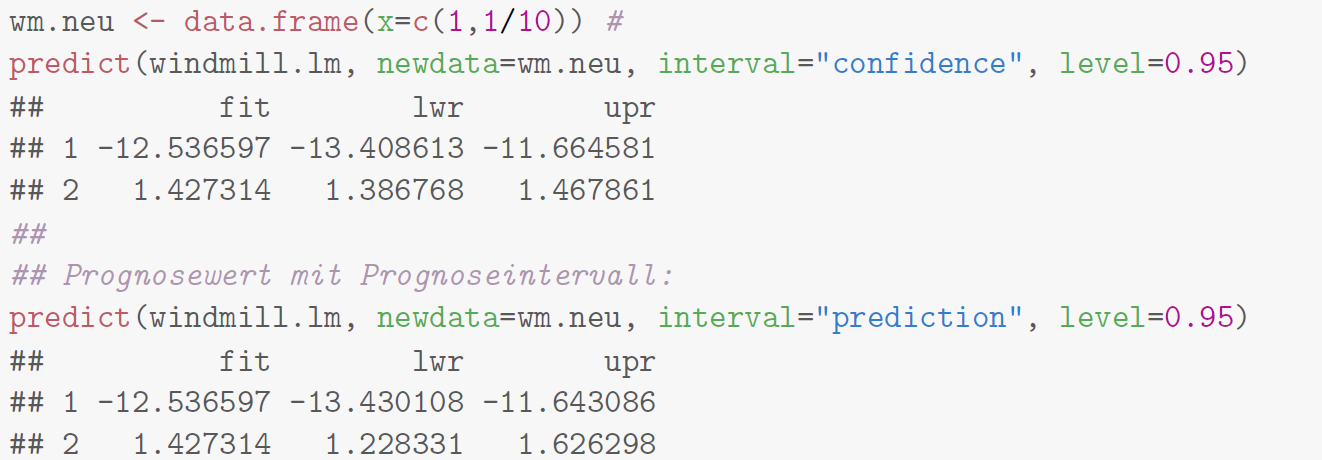
\includegraphics[width=0.5\linewidth]{./figures/Rprediction}
	\caption{\textit{Quelle:} \cite{C:Prediction}}
	\label{fig:rprediction}
\end{figure}

\begin{itemize}
	\item [1.]\textit{data.frame(x=c(1,1/10)} erstellt Vektor x mit 1 und 0.1 ($\rightarrow$ Werte für $x_0$ )
	\item [2.]\textit{$\left[\ldots\right]$interval="confidence", level=0.95$\left.\right)$} Konfidenzintervall (Vertrauensintervall) für 95\%
	\item [3.]Obere Zeile für ersten Eintrag des Vektors (1) und untere Zeile für 2. Eintrag des Vektors
	\begin{itemize}
		\item fit = Erwartungswert, anschliessend untere und obere Grenze
		\item siehe Abbildung \ref{fig:ProgrnoseUndVertrauen} für Bedeutung der Punkte
	\end{itemize}
	\item [4.]\textit{$\left[\ldots\right]$interval="prediction", level=0.95$\left.\right)$} Konfidenzintervall für 95\%
	\begin{itemize}
		\item Liefert Prognosegrenze
	\end{itemize}
\end{itemize}

\subsubsection{Multiple Lineare Regression}
\label{subsubsec:MultipleLineareRegressionR}
\begin{figure}[!h]
	\centering
	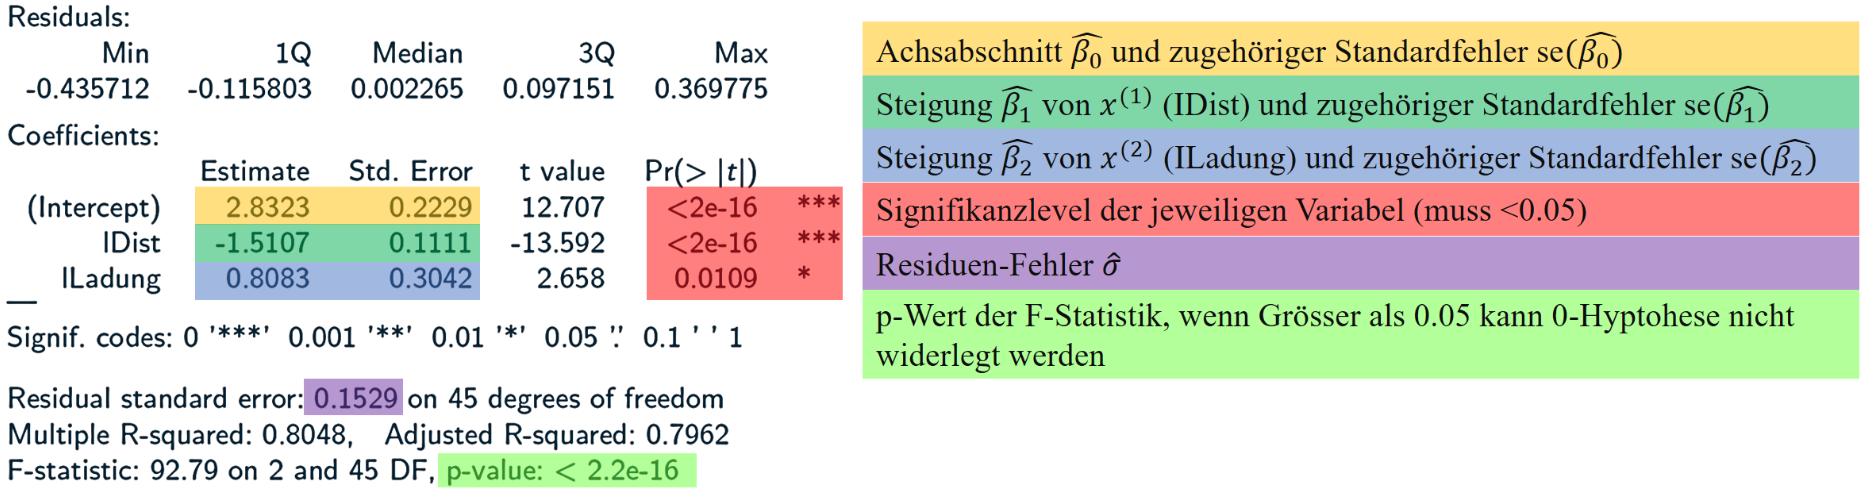
\includegraphics[width=1\linewidth]{figures/MultiReg1}
	\caption{R-Output der Multiplen Regression}
	\label{fig:multireg1}
\end{figure}


\subsubsection{Konfidenzintervall}
\label{subsubsec:konfidenzintervallR}
\begin{itemize}
	\item 95\% Intervall für jeden der Parameter
	\begin{itemize}
		\item Somit Werte mögliche Werte der Variablen damit zwischen 2.5\% und 97.5\% 
	\end{itemize}
	\item \textit{confint(lm-objekt, parm=2,level=confLvl)} würde Parameter log10(dist) als Returnwert geben
\end{itemize}
\begin{figure}[!h]
	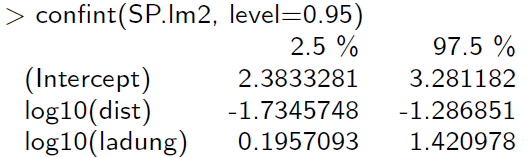
\includegraphics[width=0.3\linewidth]{figures/confint}
	\caption{Beispiel für Konfidenzintervall hier 95\%, \textit{Quelle:} \cite{C:confint}}
	\label{fig:confint}
\end{figure}

\subsubsection{Robuster Schätzer (MM-Schätzer) roblm}
\label{subsubsec:RobSchaetzer}
\begin{figure}[!h]
	\centering
	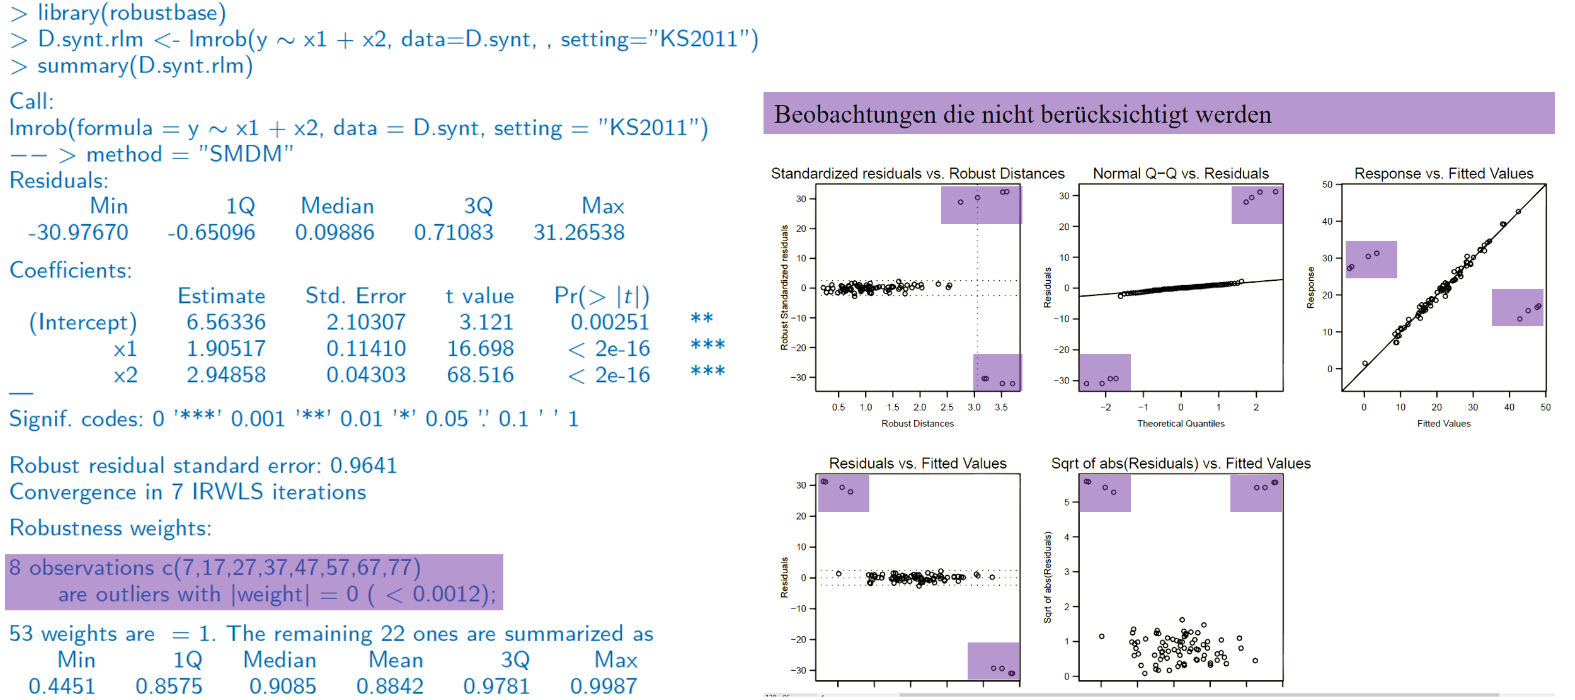
\includegraphics[width=1\linewidth]{figures/roblm}
	\caption{Output des Robusten Schätzers inkl. Zusammenhang mit den verschiedene Plots (Folie 30) \textit{Quelle:}\cite{C:Roblm}}
	\label{fig:roblm}
\end{figure}

\clearpage
\subsubsection{VIF}
\label{subsubsec:VIF}
\begin{figure}[!h]
	\centering
	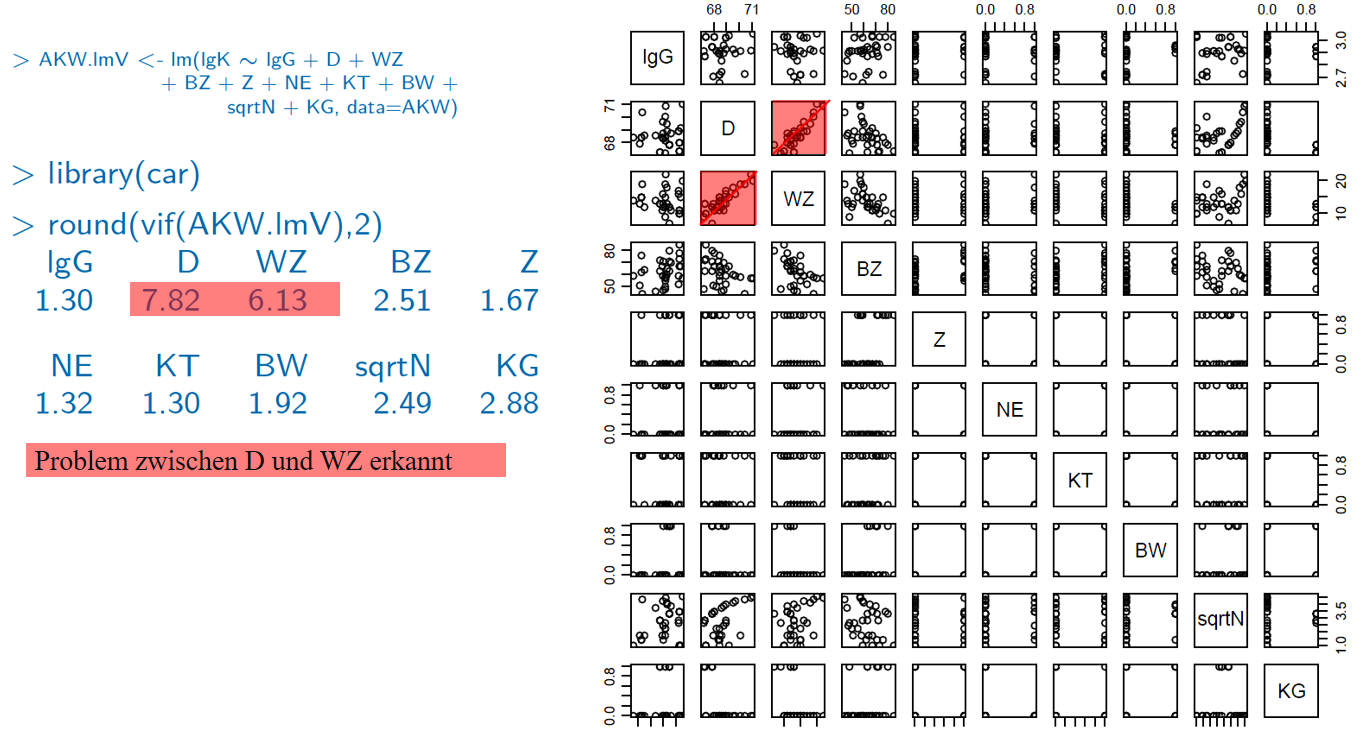
\includegraphics[width=0.9\linewidth]{figures/VIF}
	\caption{Korrelation zwischen zwei Variablen. Zu erkennen an grossem VIF-Wert und ca. linearem Verhalten wenn diese gegeneinader aufgetragen werden \textit{Quelle:} \cite{C:VIF}}
	\label{fig:vif}
\end{figure}

\subsubsection{AIC}
\label{subsubsec:AIC}
\begin{figure}[!h]
	\centering
	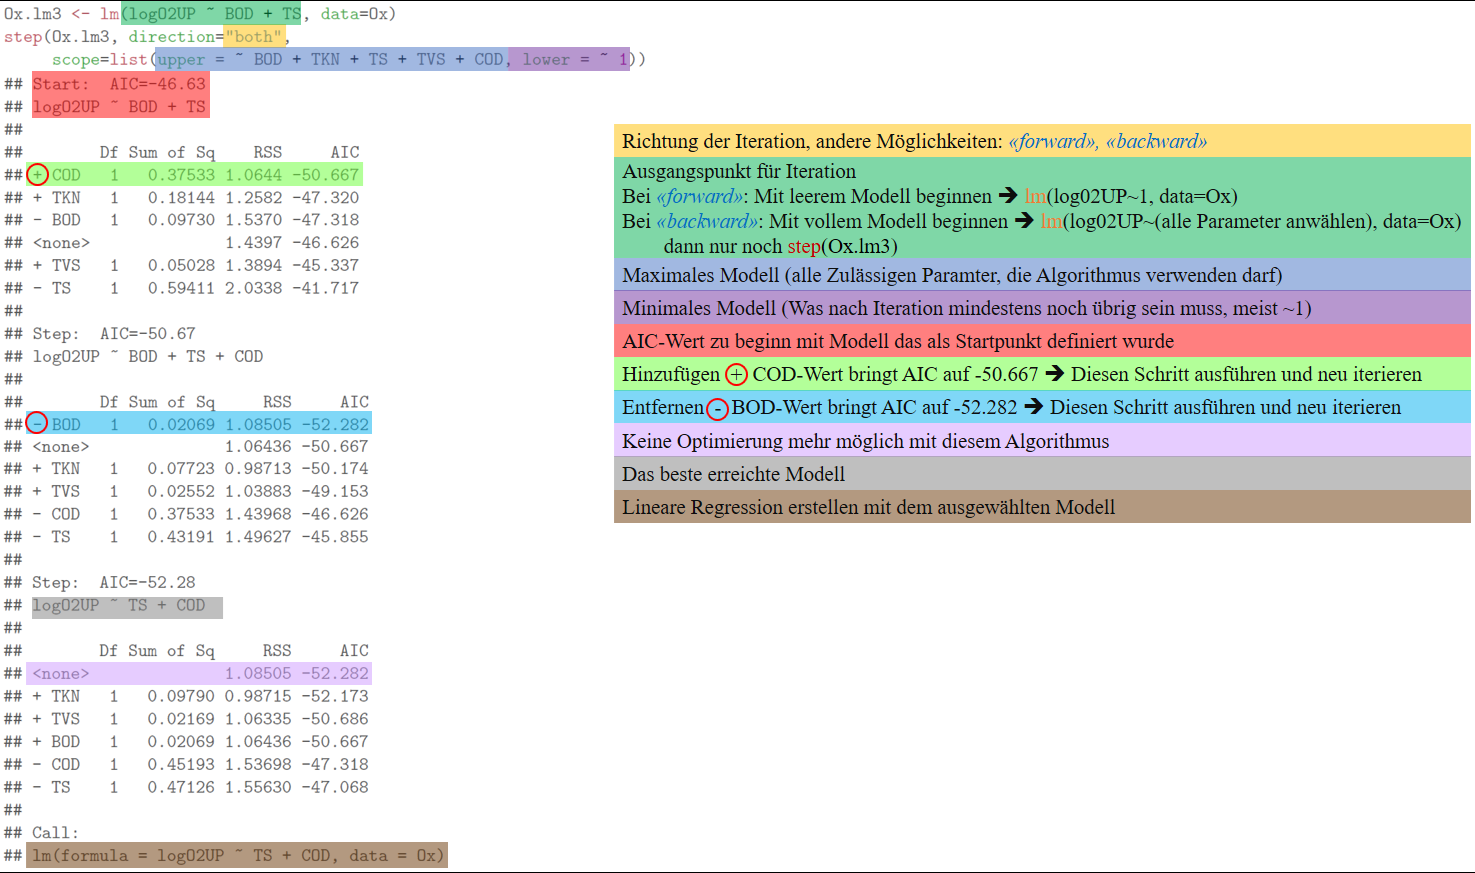
\includegraphics[width=1\linewidth]{figures/AIC}
	\caption{Output von R! für Optimierung nach AIC mit schrittweiser Selektion  \textit{Quelle:} \cite{C:AIC}}
	\label{fig:aic}
\end{figure}
\clearpage

\subsubsection{Dataframe}
\label{subsubsec:Dataframe}
\begin{figure}[h!]
	\centering
	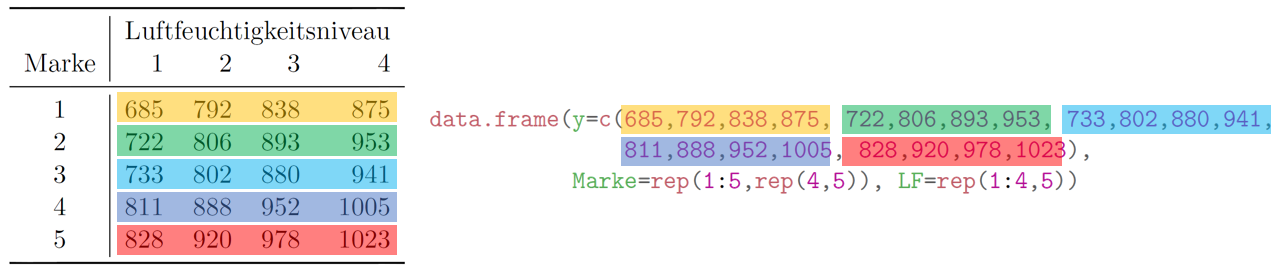
\includegraphics[width=0.7\linewidth]{figures/Dataframe}
	\caption{Manuelle Eingabe von Daten in R! \textit{Quelle:}\cite{C:dataframe}}
	\label{fig:dataframe}
\end{figure}

\clearpage
\printbibliography
\newpage
\section{Appendix}
\subsection{Tafel: standardisierten Normalverteilung \cite{C:LookUpTable}}
\begin{minipage}{0.9\linewidth}
	\label{Anh:TafelStandardisierteNormalverteilung}
	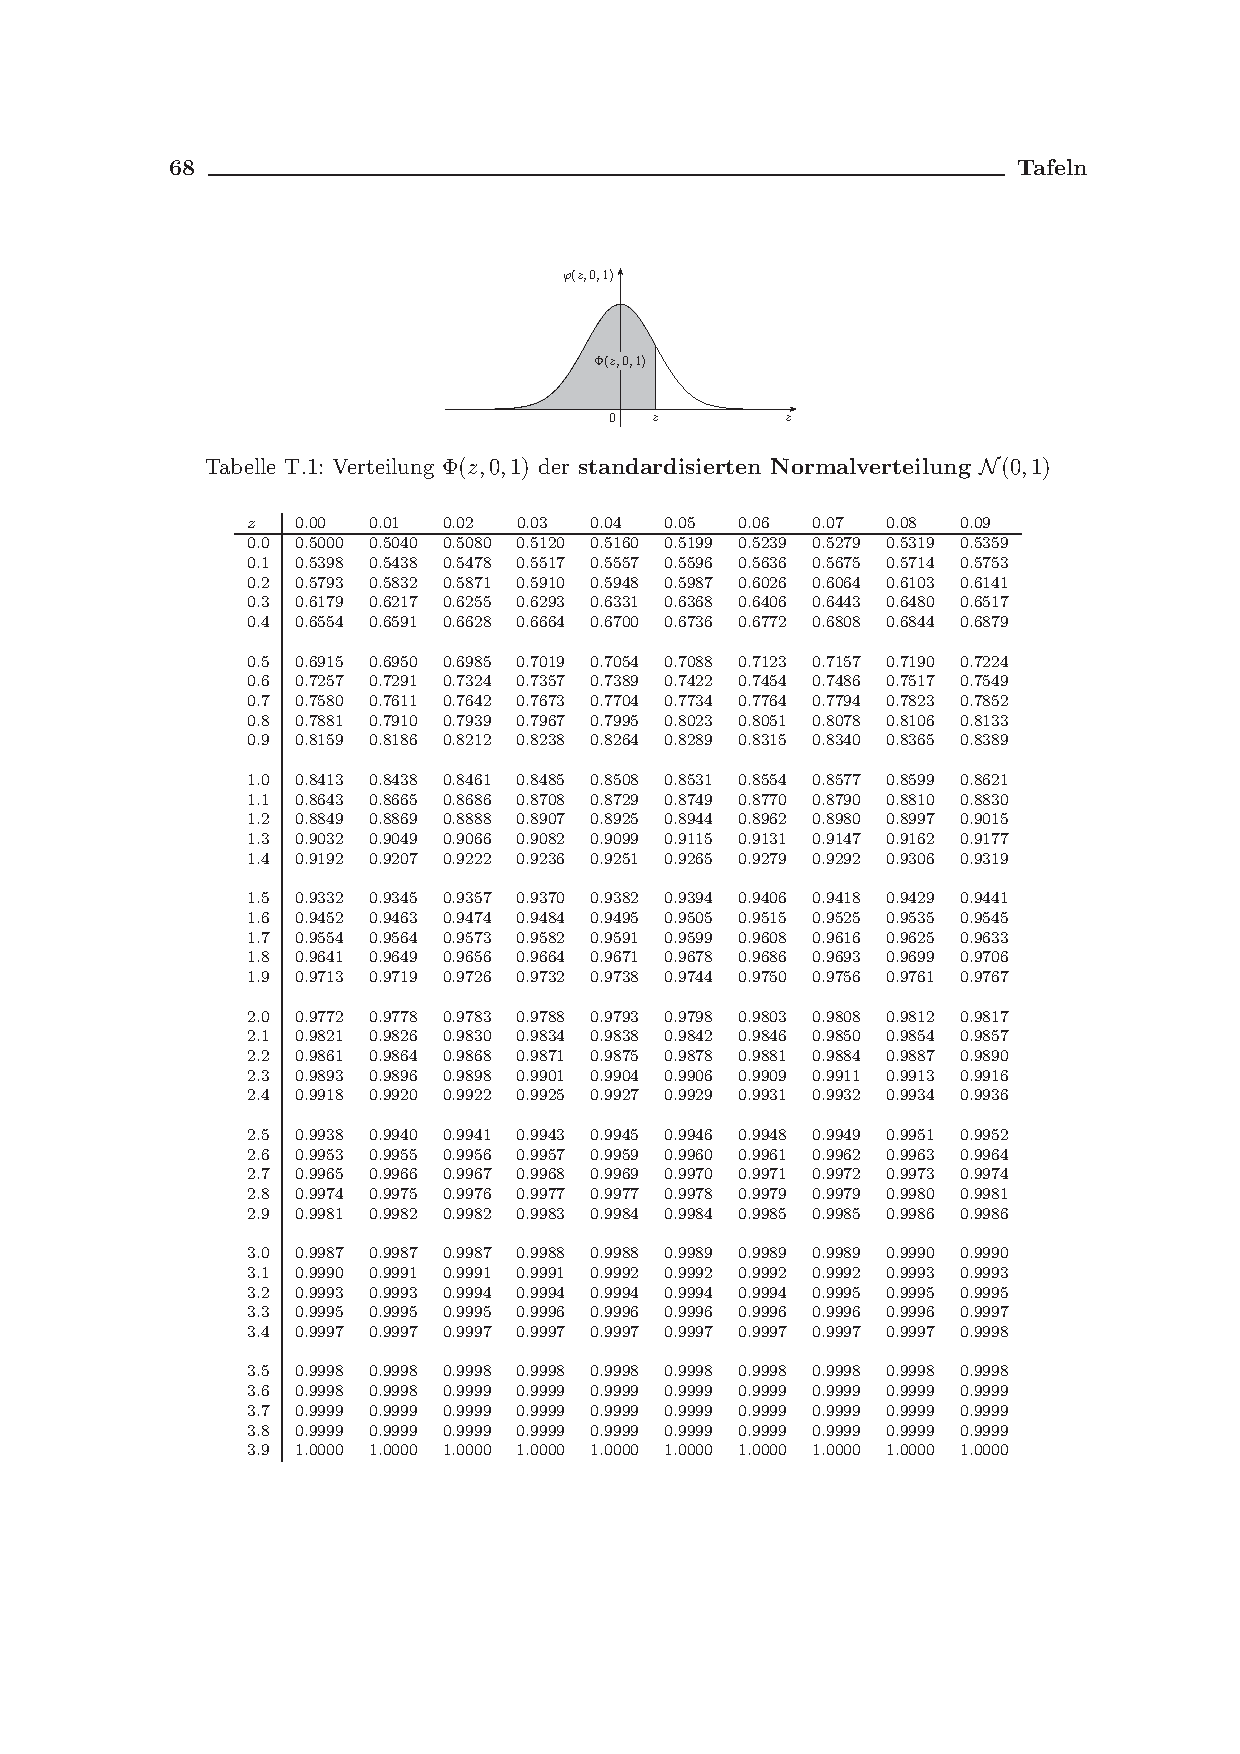
\includepdf[pages=1, trim=30mm 30mm 30mm 50mm,clip, offset = 0mm -25mm, scale = 0.85]{./appendix/Wahrscheinlichkeitstafeln.pdf}
\end{minipage}
\newpage

\subsection{Tafel: q-Quantile standardisierten Normalverteilung \cite{C:LookUpTable}}
\begin{minipage}{0.9\linewidth}	
	\label{Anh:TafelqQuantileStandardisierteNormalverteilung}
	\includepdf[pages=2, trim=25mm 30mm 25mm 35mm,clip, offset = 0mm -5mm, scale = 0.85]{./appendix/Wahrscheinlichkeitstafeln.pdf}
\end{minipage}
\newpage

\subsection{Tafel: Student-t-Verteilung \cite{C:LookUpTable}}
\begin{minipage}{0.9\linewidth}
	\label{Anh:TafelStudentTVerteilung}
	\includepdf[pages=3, trim=25mm 30mm 25mm 35mm,clip, offset = 0mm -5mm, scale = 0.85]{./appendix/Wahrscheinlichkeitstafeln.pdf}
\end{minipage}
\newpage

\subsection{Tafel: Faktoren für Konstruktion Kontrollkarten \cite{C:KonstruktionKontrollkarte}}
\begin{minipage}{0.9\linewidth}
	\label{Anh:TafelFaktorenKontrollkarten}
	\includepdf[pages=4, trim=25mm 30mm 25mm 35mm,clip, offset = 0mm -5mm, scale = 0.85]{./appendix/Wahrscheinlichkeitstafeln.pdf}
\end{minipage}
\newpage

\subsection{Tafel: Wichtigste Werte für $\sigma$}
\label{Anh:WichtigeSigma}
\begin{minipage}{\linewidth}
\begin{center}
		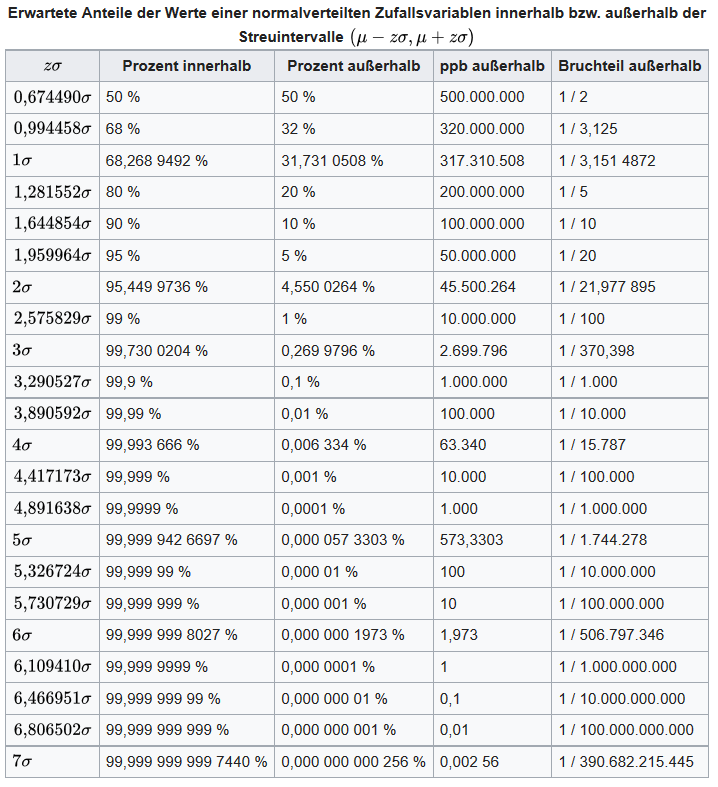
\includegraphics[width=0.8\linewidth]{figures/WichtigsteWerteSigma.png}\\
		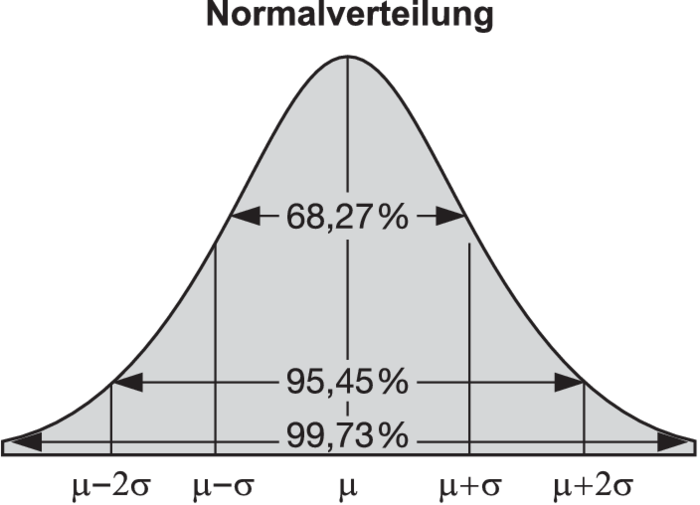
\includegraphics[width=0.3\linewidth]{figures/Normalverteilung.png}\\
		\textit{Quelle:}\cite{C:Normalverteilung}
\end{center}		

\end{minipage}

\end{document}